\chapter{\scshape KPP surface ocean boundary layer}
\label{chapter:cvmix_kpp}

\minitoc
\vspace{.5cm}

\begin{mdframed}[backgroundcolor=lightgray!50]
  This chapter summarizes the KPP scheme as implemented in CVMix for
  the ocean surface boundary layer \citep{LargeKPP}.  The following
  CVMix Fortran module is directly connected to the material in this
  chapter:
\begin{align*} 
 & {\tt cvmix\_kpp.F90}
\end{align*}
\end{mdframed}


\section{Elements of the K-profile parameterization (KPP)}
\label{sec:implementation}

The ocean surface boundary layer (OBL) mediates the exchange of
properties between the ocean and other components of the climate
system. Hence, parameterization of processes active in the OBL are
fundamental to the integrity of a climate simulation. The K-profile
parameterization (KPP) is a widely used method for parameterizing
boundary layer processes in both the atmosphere and ocean. The paper
by \cite{LargeKPP} introduced this scheme to the ocean community for
use in parameterizing processes in the surface ocean boundary layer .
The pedagogical lectures by \cite{LargeKPP_lectures} and
\cite{Large2012} provide added insight into the scheme that
complements some of the material in \cite{LargeKPP}.

The KPP scheme has been used by many ocean climate studies for
parameterizing mixing in the OBL, with examples discussed in
\cite{Largeforcing}, \cite{HollandChowBryan1998},
\cite{Gent_etal_1998}, \cite{GOTM}, \cite{LiChowMcWilliamsFu2001},
\cite{Smyth_etal2002}, \cite{Durski_etal2004}, and
\cite{Chang_etal2005}).  We consider here only the implementation of
KPP for the surface ocean boundary layer, as implementations for the
bottom do not exist in MOM or POP.



\subsection{Conventions}

We use the following conventions that are consistent with
\cite{LargeKPP} and \cite{LargeKPP_lectures}.

\begin{itemize}
 
\item The fluid is assumed to be volume conserving Boussinesq, with
  extensions to a mass conserving non-Boussinesq fluid trivial.

\item \label{geopotential_defined} The geopotential coordinate, $z$,
  which increases up and where $z=0$ defines the resting ocean
  surface. The ocean free surface is defined by $z=\eta(x,y,t)$ and
  the static ocean bottom is at $z=-H(x,y)$.

\item \label{lambda_defined} A lowercase $\lambda$ is used to denote
  a turbulent fluctuation of an arbitrary field within the surface
  ocean boundary layer; e.g., a tracer such as potential or
  conservative temperature $\theta$ and salinity $s$), or a velocity
  component ($u,v,w$). Note that $x$ is the notation used in
  \cite{LargeKPP} and \cite{LargeKPP_lectures}, but we prefer the
  Greek letter $\lambda$ to avoid confusion with the horizontal
  spatial coordinate.

\item \label{Lambda_defined} An uppercase $\Lambda$ is used to denote
  the Eulerian mean of a tracer or velocity component within the
  surface ocean boundary layer; e.g., potential or conservative
  temperature $\Theta$, salinity $S$, or velocity component ($U,V,W$).
  The Eulerian mean fields are time stepped by an ocean climate model
  within the boundary layer, and correlations of turbulent variables
  must be parameterized to close the mean field equations.

\item \label{correlation_defined} The expression $\overline{w \,
    \lambda}$ is used to symbolize the Eulerian correlation of the
  fluctuating turbulent vertical velocity and a fluctuating scalar or
  vector field. This correlation appears in the mean field time
  tendency equation for $\Lambda$ in the Boussinesq primitive ocean
  equations (see equation (\ref{eq:mean-field-equation-kpp})). KPP
  provides a parameterization of this vertical turbulent flux within
  the surface ocean boundary layer.

\item \label{w_W_defined} The mean and turbulent vertical velocity
  components, $W,w$, are positive for upward motion. This sign
  convention implies that
   \begin{equation}
  \overline{w \, \lambda}   > 0  \implies \mbox{turbulent flux for $\lambda$ transported vertically upward}.
\label{eq:correlation-convention}
\end{equation}
If $\lambda$ is the temperature, then a positive correlation at the
ocean surface, $\overline{w \, \theta}^{\eta} > 0$, corresponds to
surface cooling.

\end{itemize}

 
\subsection{General form of the parameterization}

Ignoring all terms except vertical advective transport in the
prognostic equation for the mean field $\Lambda$, its time tendency 
is determined by 
\begin{equation}
 \frac{\partial \Lambda}{\partial t} = -\left( \frac{\partial \, (W \, \Lambda)}{\partial z} \right)  
 -\left( \frac{\partial \, (\overline{w \, \lambda}) }{\partial z} \right).  
\label{eq:mean-field-equation-kpp}
\end{equation}
The advective flux by the mean vertical velocity, $W \, \Lambda$, is
represented via a numerical advection operator. In contrast, the
turbulent correlation, $\overline{w \, \lambda}$, is a subgrid scale
flux that must be parameterized in order to close the equation for
$\Lambda$. Here, the overbar signifies an Eulerian averaging operator
over unresolved turbulent motions occurring within the OBL.

The KPP scheme provides a first order closure for $\overline{w \,
  \lambda}$ within the OBL. It does so by introducing two terms in the
following manner 
\begin{equation}
  \overline{w \, \lambda} = -K_{\lambda} \left( \frac{\partial \Lambda}{\partial z} - \gamma_{\lambda} \right).
\label{eq:kpp-parameterization}
\end{equation}
The KPP prescription (\ref{eq:kpp-parameterization}) thus
parameterizes the vertical turbulent flux using two terms
\begin{equation}
  \overline{w \, \lambda} = \overline{w \, \lambda}^{\mbox{\tiny local}} + \overline{w \, \lambda}^{\mbox{\tiny non-local}}.
\label{eq:vertical-flux-decomposed}
\end{equation}
The first term provides for the familiar downgradient vertical
diffusion determined by a vertical diffusivity and the local vertical
derivative of the mean field.  This term is referred to as the local
portion of the parameterization
\begin{equation}
\overline{w \, \lambda}^{\mbox{\tiny local}} = -K_{\lambda} \left( \frac{\partial \Lambda}{\partial z} \right).
\label{eq:vertical-flux-local}
\end{equation}
Note that the diffusivity computed from KPP is a non-local function of
boundary layer properties, so the name ``local'' is not directed at
the diffusivity, but instead at the vertical derivative.  The second
term, $\gamma_{\lambda}$, accounts for non-local transport that is not
directly associated with local vertical gradients of $\Lambda$, in
which
\begin{equation}
\overline{w \, \lambda}^{\mbox{\tiny non-local}} = K_{\lambda} \; \gamma_{\lambda}.
\label{eq:vertical-flux-nonlocal}
\end{equation}
We next provide a general discussion of these two contributions to the
KPP parameterization.


\subsection{The vertical diffusivity}
\label{subsection:kpp-vertical-diffusivity}

The vertical diffusivity arising from KPP in the OBL is determined as
a non-local function of boundary layer properties. It is written in
the following form
\begin{equation}
  K_{\lambda}(\sigma) = h \, w_{\lambda}(\sigma) \, G_{\lambda}(\sigma).
\label{eq:kpp-diffusivity}
\end{equation}
The diffusivity is a constructed as the product of three terms: the
boundary layer thickness $h$, the vertical turbulent velocity scale
$w_{\lambda}(\sigma)$, and the vertical shape function
$G_{\lambda}(\sigma)$.  Note that we introduce a dependence of the
shape function on the field diffused.  As discussed in Section
\ref{subsection:kpp-shape-function}, this dependence arises from
matching to interior diffusivities, which are generally a function of
$\lambda$.


\subsubsection{Boundary layer thickness} 

The boundary layer thickness is denoted by 
\begin{equation}
 h \ge 0 \; \; \mbox{is the boundary layer thickness}.
\label{eq:boundary-layer-thickness}
\end{equation}
This is the thickness of the OBL prescribed by the KPP scheme, with
details given in Section \ref{subsection:kpp-obl-thickness}. The
direct dependence of the vertical diffusivity in equation
(\ref{eq:kpp-diffusivity}) on the OBL thickness manifests the common
property of boundary layers, whereby thicker layers generally arise
from stronger eddy motions and are thus associated with more rapid
mixing of tracer concentration and momentum.

Figure \ref{fig:boundary-layer-schematic-kpp} provides a schematic of
the KPP boundary layer, the Monin-Obukhov surface layer, and the
associated momentum, mass, and buoyancy fluxes impacting these layers.
Details of this figure will be explored in the following.



\subsubsection{Measuring vertical distances within the OBL}

When measuring distances within the boundary layer, it is the
thickness of the water as measured from the ocean surface that is
important. Free surface undulations can be a nontrivial fraction of
the boundary layer thickness, particularly under conditions of stable
buoyancy forcing. Hence, we make explicit note that the ocean has an
undulating free surface at $z=\eta(x,y,t)$, which contrasts to
\cite{LargeKPP} and \cite{LargeKPP_lectures}, who assumed that $z=0$
sets the upper ocean surface.

Following \cite{LargeKPP}, we introduce the non-dimensional depth,
$\sigma$, given by 
\begin{equation}
  \sigma = \frac{d}{h}.
\label{eq:sigma-defined}
\end{equation}
In this definition, $d \ge 0$ is the distance from the ocean surface
at $z=\eta$ to a point within the boundary layer
\begin{equation}
  d = -z+\eta.
\label{eq:distance-from-surface-defined}
\end{equation}
Likewise, $h \ge 0$ is the distance from the free surface 
to the bottom of the boundary layer
\begin{equation}
  h = h_{\mbox{\tiny obl}} +\eta,
\label{eq:h-obl-defined}
\end{equation}
where $h_{\mbox{\tiny obl}}$ is the depth of the boundary layer as
measured from $z=0$. That is, $h$ is the thickness of the OBL, and it is this 
thickness, not $h_{\mbox{\tiny obl}}$, that is
predicted  by KPP (Section \ref{subsection:kpp-obl-thickness}).
Regions within the boundary layer are given by the non-dimensional
depth range
\begin{equation}
  0 \le \sigma \le 1 \qquad \mbox{within boundary layer,}
\end{equation}
with $\sigma=0$ the ocean surface and $\sigma = 1$ the bottom of the
boundary layer.



%%%%%%%%%%%%%%%%%%%% %%%%%%%%%%%%%%%%%%%%%%%%%
\begin{figure}[h!t]
\rule{\textwidth}{0.005in}
\begin{center}
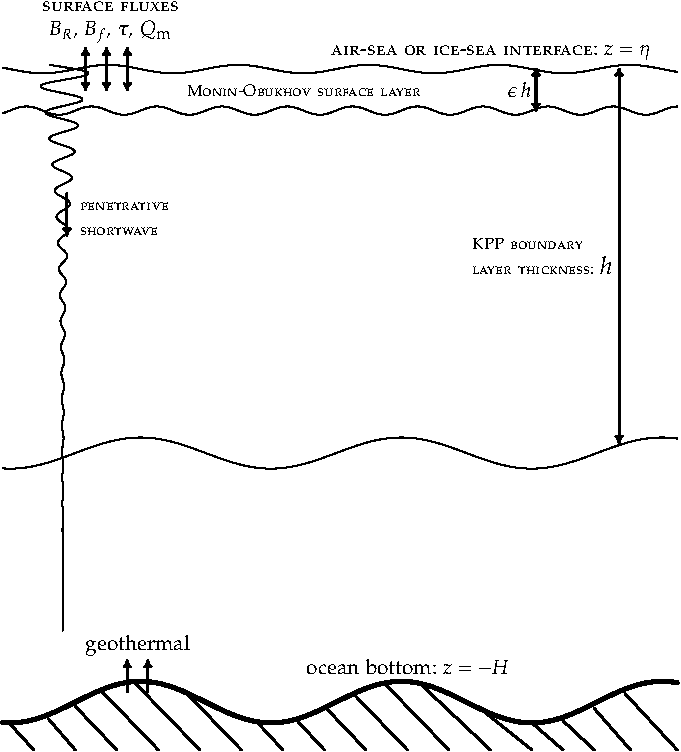
\includegraphics[angle=0,width=10cm]{./mfpic_figs/cvmix_kpp_boundary_layer.pdf}
\caption[KPP boundary layer schematic]{\sf Schematic of the upper
  ocean boundary layer regions associated with the KPP boundary layer
  parameterization.  The upper ocean is exposed to non-penetrative
  air-sea and ice-sea fluxes of momentum $\bftau$ (Section
  \ref{section:boundary-forcing-momentum-kpp}), mass $\Qm$(Section
  \ref{section:boundary-forcing-buoyancy-kpp}), and buoyancy $B_{f}$
  (Section \ref{section:boundary-forcing-buoyancy-kpp}).  In addition,
  there is penetrative shortwave radiation, $-\overline{w \,
    \theta}_{R}$ (Section
  \ref{section:boundary-forcing-buoyancy-kpp}), indicated by the
  exponentially decaying vertical sinusoidal.  The Monin-Obukhov
  surface layer (Section \ref{section:m-o-similarity}) has a thickness
  $\epsilon \, h$, with $\epsilon \approx 0.1$.  The surface layer is
  where turbulence delivers fluxes to the molecular skin layer for
  transfer to the atmosphere or ice.  The surface layer starts from
  just beneath the surface roughness elements at the upper ocean
  interface.  Since neither these roughness elements, nor the
  molecular viscous sublayer, are resolved in ocean models, we assume
  in practice that the Monin-Obukhov surface layer extends to the sea
  surface at $z=\eta(x,y,t)$.  The KPP boundary layer includes the
  surface layer, and it has a thickness $h(x,y,t)$ determined by the
  KPP parameterization (Section \ref{subsection:kpp-obl-thickness}).
  The ocean bottom at $z=-H(x,y)$ is rigid and is exposed to
  geothermal heating.  Presently, the KPP boundary layer scheme has
  not been implemented in MOM or POP to parameterize bottom boundary
  layer physics, though nothing fundamental precludes such.  In fact,
  \cite{Durski_etal2004} provide just such an implementation.}
\label{fig:boundary-layer-schematic-kpp}
\end{center}
\rule{\textwidth}{0.005in}
\end{figure}
%%%%%%%%%%%%%%%%%%%%%%%%%%%%%%%%%%%%%%%%%%%%%%%%%%%%%%%%%%%%%%%%%%%%%%%%



\subsubsection{Scale for turbulent vertical velocity fluctuations: $w_{\lambda}$}
\label{subsubsection:turbulent-vertical-velocity-scale}

Scale for turbulent vertical velocity fluctuations is written
$w_{\lambda}$.  It is a function of depth within the boundary layer,
and a function of the field to which it refers. We return to its
specification in Section \ref{subsection:vertical-velocity-scale}.


\subsubsection{Non-dimensional vertical shape function $G_{\lambda}(\sigma)$}

Non-dimensional vertical shape function $G_{\lambda}(\sigma)$ is used to
smoothly transition from the ocean surface to the bottom of the
boundary layer. \cite{LargeKPP} chose a cubic polynomial
\begin{equation}
 G_{\lambda}(\sigma) = a_{0} + a_{1} \, \sigma + a_{2} \, \sigma^{2} + a_{3} \, \sigma^{3}.
\label{eq:structure-function-gsigma}
\end{equation}
Since turbulent eddies do not cross the ocean surface at $\sigma=0$,
we should correspondingly have a vanishing diffusivity at $\sigma=0$.
This constraint is satisfied by setting 
\begin{equation}
 a_{0} = 0.
\end{equation}
We detail in Section \ref{subsection:kpp-shape-function} how to
specify the remaining expansion coefficients $a_{1}, a_{2}, a_{3}$.
In particular, we simplify the specification of \cite{LargeKPP}.


\subsection{The non-local transport $\gamma_{\lambda}$}
\label{subsection:kpp-nonlocal-transport-outline}

There are many processes in the boundary layer that lead to transport
that is difficult to parameterize a a function of the local vertical
derivative of the mean field (see Section 2 of \cite{LargeKPP}).  This
behaviour leads to a diffusivity $K_{\lambda}$ that is a function of
the surface fluxes and boundary layer thickness $h$.  Furthermore,
under convective forcing (negative surface buoyancy forcing; $B_{f} <
0$), fluxes can penetrate into stratified interior.  This
characteristic then motivates the introduction of a non-local
transport term $\gamma_{\lambda}$ to the KPP parameterization
(equation (\ref{eq:kpp-parameterization})) when $B_{f} < 0$.  To
further identify the need for a non-local transport term
$\gamma_{\lambda}$, we reproduce Figure 1 from \cite{LargeKPP}, here
shown as Figure \ref{fig:kpp-figure1-reproduced}.  The caption to
Figure \ref{fig:kpp-figure1-reproduced} explores the many facets of
this figure used to help justify the non-local term in KPP.

%%%%%%%%%%%%%%%%%%%% %%%%%%%%%%%%%%%%%%%%%%%%%
\begin{figure}[h!t]
\rule{\textwidth}{0.005in}
\begin{center}
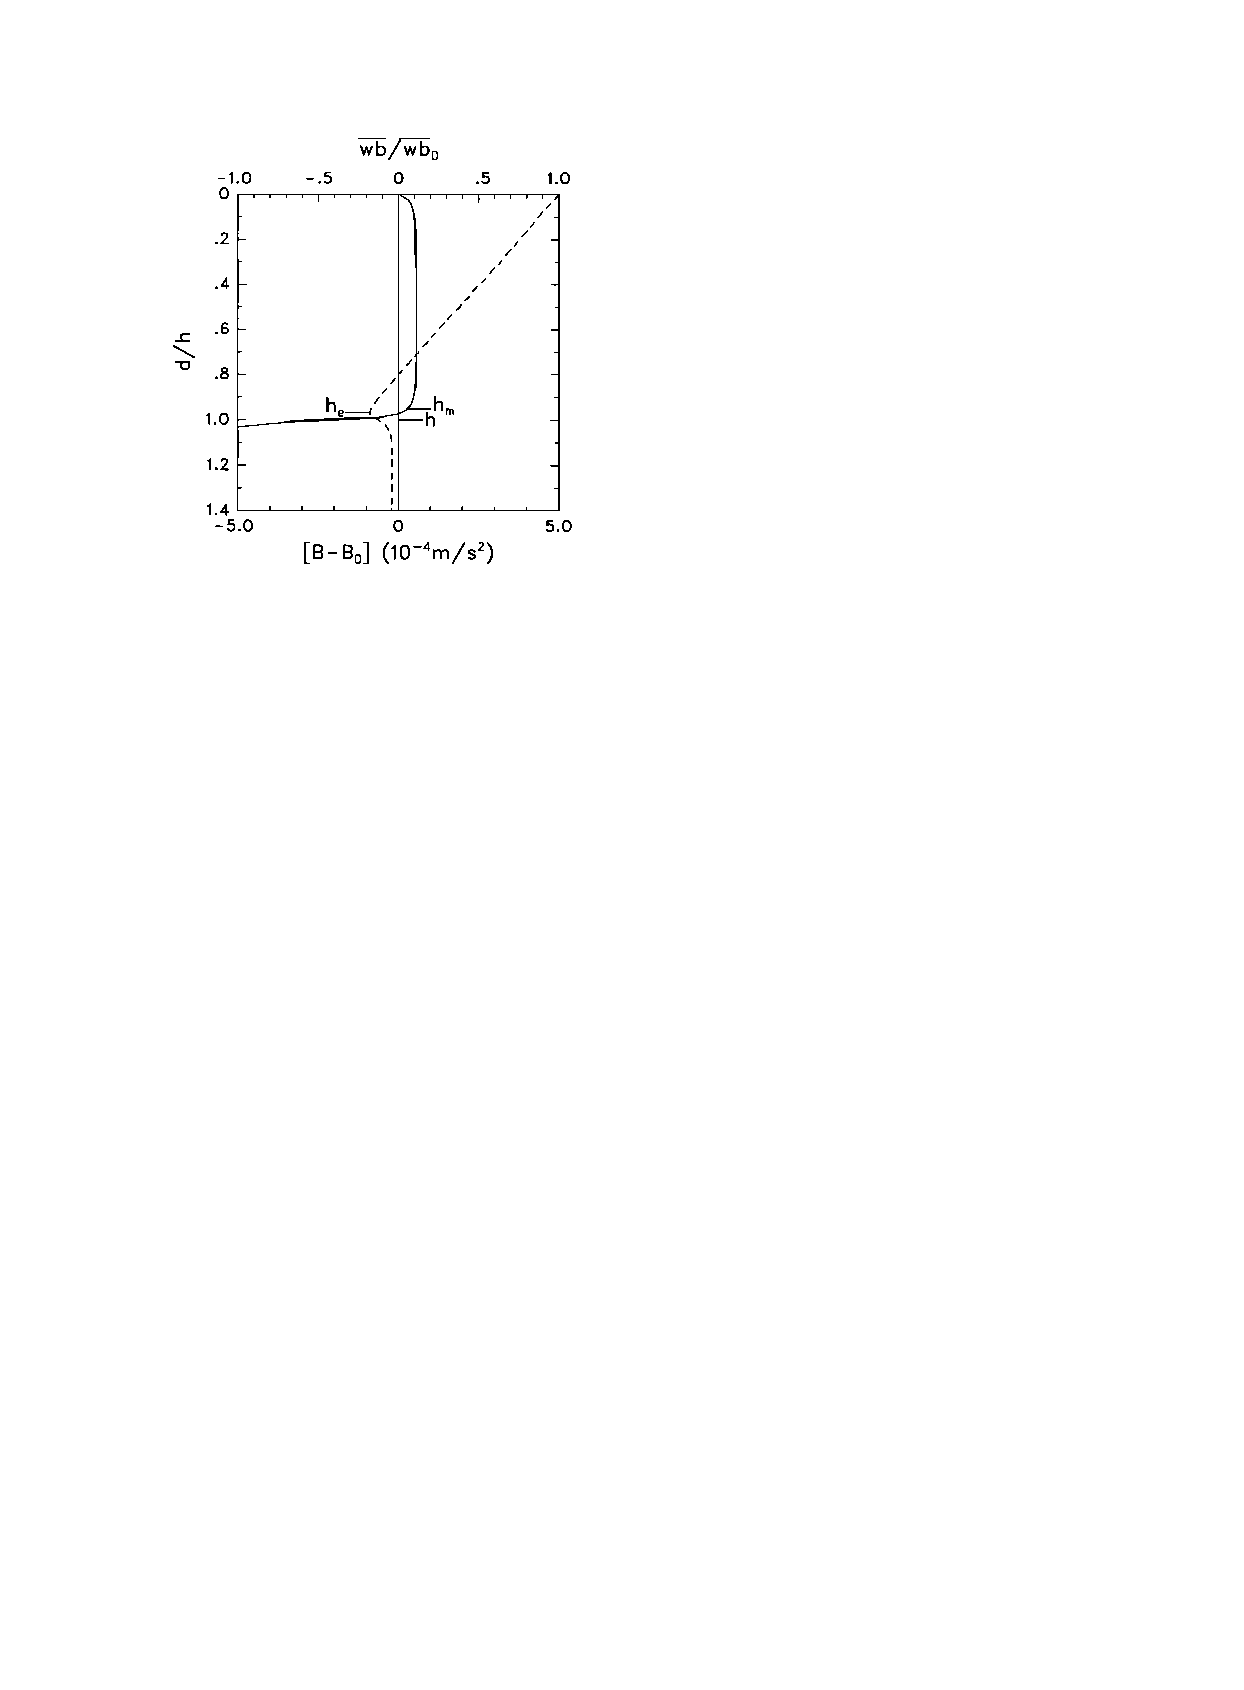
\includegraphics[angle=0,width=10cm]{./figs/LargeKPP_fig1.pdf}
\caption[Figure 1 from \cite{LargeKPP}]{
  \sf
This is a reproduction of
  Figure 1 from \cite{LargeKPP}.
  The figure is derived from a one-dimensional simulation after 3 days of
  convective deepening (zero winds; negative surface buoyancy forcing)
  into an initially uniformly  stratified water column.  The vertical axis
  is vertical distance starting from the ocean surface interface at
  $z=\eta$ and $d=0$, extending down to $d=h$ ($h=13.6$~m at this point
  of the integration), which is the base of
  the boundary layer, and finally to $d=1.4\, h$, which is beneath the
  boundary layer.

 \hspace{0.4cm} The horizontal axis on the bottom is the mean buoyancy, $B$,
  relative to that at the surface, $B_{0}$, and the profile is
  depicted by the solid line. Positive values of
  $B-B_{0}$ indicate that the mean buoyancy at a point is larger than 
  at the surface, with $B-B_{0} > 0$ expected under
  negative buoyancy forcing at the ocean surface.  

  \hspace{0.4cm}  The horizontal axis on
  the top is the ratio of the local turbulent buoyancy flux
  $\overline{w \, b}$ to the surface turbulent flux $\overline{w \,
    b}^{\eta}$ (denoted $\overline{w \, b}_{0}$ by \cite{LargeKPP}).
  The dashed line depicts this ratio.  Positive values of $\overline{w
    \, b}$ represent upward turbulent buoyancy fluxes; e.g., upward
  fluxes of heat for the case where buoyancy is determined by
  temperature, and the thermal expansion coefficient is positive.
  
  \hspace{0.4cm}  Positive values for $\overline{w \, b}$  in regions between roughly $0.35 < d
  < 0.8$ represent upward turbulent buoyancy fluxes in a region where the mean vertical
  gradient of $B$ is nearly zero, thus indicating non-local turbulent transport.
  In shallower regions with $d < 0.35$, the mean gradient is negative,
  $\partial_{z} B < 0$, and the fluxes are positive, $\overline{w \,
    b} > 0$, thus representing downgradient turbulent fluxes.
  Likewise, for $d> 0.8$, the turbulent fluxes are downgradient.

  \hspace{0.4cm} The mixed layer depth is denoted by $h_{m}$, though
  this depth is subject to arbitrary specification of the density
  difference. The entrainment depth is $h_{e}$, with this depth taken
  where the buoyancy flux reaches a negative extrema. Note that it is
  an empirical result that under pure convective forcing ($\bftau =0,
  B_{f} < 0$), the turbulent entrainment flux is roughly 20\% of the
  surface flux: $\overline{w \, b}^{d=h_{e}} = \beta_{T} \;
  \overline{w \, b}^{d=0}$, where $\beta_{T} = -0.2$. This situation
  is depicted in the figure. }
\label{fig:kpp-figure1-reproduced}
\end{center}
\rule{\textwidth}{0.005in}
\end{figure}
%%%%%%%%%%%%%%%%%%%%%%%%%%%%%%%%%%%%%%%%%%%%%%%%%%%%%%%%%%%%%%%%%%%%%%%%


As part of the KPP parameterization, the non-local transport,
$\gamma_{\lambda}$, aims to account for such processes as boundary
layer eddies whose transport may be unrelated to the local vertical
gradient of the mean field, and whose impacts may penetrate within the
stratified ocean interior. In general, \cite{LargeKPP} prescribe the
following characteristics to $\gamma_{\lambda}$.
\begin{itemize}

\item Page 371 of \citep{LargeKPP} notes that there is no theory for
  non-local momentum transport, and so the non-local transport
  directly affects only the tracer fields:
\begin{equation}
 \gamma_{\lambda} \; \; = \; \; 
\left\{
 \begin{array}{ll}
  0 \; \;  &\mbox{if $\lambda = (u,v,w)$ a velocity component}
 \\
  \ne 0 \; \; &\mbox{nonzero if $\lambda = \theta,s$ or another tracer.}
  \end{array}
 \right.
\end{equation}
However, \cite{Smyth_etal2002} consider a non-local term for momentum,
thus motivating further research to see whether it is suitable for
climate modeling.  

  \item The non-local transport is non-zero only within the OBL:  
\begin{equation}
 \gamma_{\lambda} \; \; = \; \; 
  \left\{ 
  \begin{array}{ll}
   0 \; \; &\mbox{if $\sigma > 1$}
   \\ 
   \ne 0  \; \; &\mbox{if $0 \le \sigma \le 1$.}
  \end{array}
 \right.
\end{equation}

  \item The non-local transport is non-zero only in the presence of
    destabilizing negative surface ocean buoyancy flux, whose presence
    gives rise to convective mixing:
\begin{equation}
 \gamma_{\lambda} \; \; = \; \; 
  \left\{ 
  \begin{array}{ll}
   0 \; \; &\mbox{for positive (stabilizing) surface buoyancy forcing}
   \\ 
   \ne 0  \; \; &\mbox{for negative (destabilizing) surface buoyancy forcing.}
  \end{array}
 \right.
\end{equation}

  \item The non-local transport can give rise, under
    certain conditions, to either down-gradient or up-gradient
    transport of the mean tracer field. Hence, it can either act to
    smooth gradients of mean fields (downgradient non-local fluxes) or
    enhance gradients (upgradient non-local fluxes).

\end{itemize}
We summarize the KPP parameterization of $\gamma_{\lambda}$ in Section
\ref{subsection:kpp-non-local-transport}.



\section{Surface ocean boundary momentum fluxes}
\label{section:boundary-forcing-momentum-kpp}

In this section and Section
\ref{section:boundary-forcing-buoyancy-kpp}, we present features of
how surface boundary fluxes force the upper ocean, largely following
Appendix A of \cite{LargeKPP}.  The aim is to identify how surface
boundary fluxes impact the upper ocean, with this characterization
then used in Section \ref{section:m-o-similarity} to help establish
some basic features of ocean boundary layers.  These ideas are then
used in Section \ref{section:specifying-kpp-diffusivity-nonlocal} to
specify the diffusivity and non-local transport from the KPP
parameterization.

Vertical exchange of momentum across the atmosphere-ocean or
sea-ice-ocean boundary occurs largely through turbulent processes.
The resulting horizontal stress vector acting on the ocean, $\bftau$,
is determined through application of a bulk formula \citep[e.g., see
Appendix C of][]{CORE_NYF}. For our purposes, we assume $\bftau$ is given,
thus yielding the ocean kinematic fluxes associated with the turbulent
transport of momentum across the ocean surface
\begin{equation}
 -\overline{w \, {\bf u}}^{\eta} 
 = \left( \frac{ \bftau }{\rho(\eta)} \right) \approx \left( \frac{ \bftau }{\rho_{0}} \right).
\label{eq:wu-kinematic-flux-kpp}
\end{equation} 
In this equation, $\rho(\eta)$ is the surface ocean density, which is
commonly approximated by the constant Boussinesq reference density
$\rho_{0}$.  A positive sign on a component of $\bftau$ acts to
accelerate the flow in the respective direction, whereas a positive
sign to a component of $\overline{w \, {\bf u}}^{\eta}$ removes
momentum from the ocean.  These sign conventions give rise to the
minus sign in the relation (\ref{eq:wu-kinematic-flux-kpp}).  In
addition to defining the kinematic surface fluxes, knowledge of
$\bftau$ allows us to compute surface boundary layer velocity scales
when working within the Monin-Obukhov similarity theory (Section
\ref{subsection:m-o-similarity-theory}).

In addition to turbulent momentum transfer, $\bftau$ is associated
with momentum transported through mass exchange across the ocean
surface, since water transported across the ocean generally carries a
nonzero momentum.  \cite{KanthaClaysonII} (see their page 431) point
out that this effect can be nontrivial, particularly when resolving
strong atmospheric storms. They also make the case for including this
effect in computing the Monin-Obukhov length scale defined by equation
(\ref{eq:m-o-length-scale})) (see their equation (4.3.11)).  Notably,
when running a coupled model, the stress from rain is included, since
it is part of the momentum convergence acting at the bottom of the
atmospheric column.  Modifying the stress from a prescribed
atmospheric state, such as CORE \citep{LargeYeager2009}, requires
further considerations.


\section{Surface ocean boundary buoyancy fluxes}
\label{section:boundary-forcing-buoyancy-kpp}

Turbulent and advective fluxes of momentum and buoyancy are
transferred across the upper ocean surface boundary, with ocean
processes such as advection and mixing then transporting the boundary
momentum and buoyancy laterally as well as into the ocean interior.
In contrast, penetrative shortwave radiation is absorbed into the
ocean absent ocean transport processes, with such absorption a
function of ocean optical properties.  In the unphysical case of
perfectly transparent seawater, shortwave radiation penetrates through
the boundary layer and so has no influence on boundary layer
processes.  In realistic cases, much of the shortwave radiation is
absorbed in the boundary layer, with only a fraction leaking through
to the interior. In general, such non-turbulent and non-advective
transport of buoyancy via penetrative radiation represents a
fundamentally novel aspect of ocean boundary layer physics relative to
the atmosphere.  Namely, for the atmosphere, radiative absorption is
far less relevant than in the upper ocean, since the atmosphere is
largely transparent to radiation.  We therefore consider penetrative
shortwave radiation as distinct from other buoyancy fluxes when
formulating how boundary fluxes impact the ocean.


\subsection{General features of buoyancy forcing}

The buoyancy of a fluid is commonly defined as (e.g., page 83 of
\cite{LargeKPP_lectures})
\begin{equation}
 B = g \, \left( \frac{ \rho_{0} - \rho}{\rho_{0}} \right), 
\label{eq:buoyancy-kpp}
\end{equation}
where $g$ is the constant gravitational acceleration, and $\rho_{0}$
is a reference density, taken here to equal the Boussinesq reference
density.  A reduction in density is associated with an increase in
buoyancy; that is, the water becomes more {\it buoyant}.  Changes in
buoyancy arise through changes in density associated with temperature
and salinity changes, since buoyancy changes are computed relative to
a fixed pressure level. In this way, buoyancy changes are directly
related to processes that impact locally referenced potential density.

Ocean buoyancy is affected through surface ocean heat, salt, and water
fluxes. 
\begin{itemize}

\item Turbulent processes transfer heat through latent and sensible
  heating.

\item Longwave radiation cools the upper ocean, with this radiation
  affected by the upper ocean skin temperature.  

\item Penetrative shortwave radiation is absorbed in seawater.

\item The transfer of salt occurs when sea ice melts and forms.  This
  transfer is proportional to the water mass flux and the difference
  in salinity between the liquid ocean and sea ice.  More generally,
  we simply consider this to be a salt flux between sea ice and ocean,
  with this flux operationally computed as part of a sea ice model.

\item Advective processes transfer heat and salt across the ocean
  surface through the transfer of water mass across the interface.

\end{itemize}
  We further detail these fluxes in the following. 


\subsection{Temperature, salinity, and mass budget for a surface
  ocean model grid cell}

Buoyancy is not a prognostic variable in ocean models.  So to develop
a quantative understanding of how buoyancy is impacted by surface
fluxes, we consider the evolution of temperature, salinity, and mass
in an arbitrary top model grid cell, and focus exclusively on
evolution arising from surface boundary fluxes.  We write these
budgets in their finite volume sense as in MOM, which includes density
and thickness weighting
\begin{align}
 \partial_{t} \, (\rho \, \mathrm{d}z \, \Theta) &=  \Qm \, \Thetam 
  - Q_{\theta}^{\mbox{\tiny non-pen}} 
  + \left( Q_{\theta}^{\mbox{\tiny pen}}(z=\eta) - Q_{\theta}^{\mbox{\tiny pen}}(z=-\Delta z) 
     \right)
 \label{eq:surface-temperature-equation-kpp}
\\
 \partial_{t} \, (\rho \, \mathrm{d}z \, S) &=  \Qm \, \Sm - Q_{S}
 \label{eq:surface-salinity-equation-kpp}
  \\
 \partial_{t} \, (\rho \, \mathrm{d}z) &=
  \Qm.
 \label{eq:surface-mass-equation-kpp}
\end{align}
 We now detail the terms appearing in these equations.  
\begin{itemize}

\item $\rho \, \mathrm{d}z$ is the mass per horizontal area of
  seawater in the grid cell.  For a volume conserving Boussinesq
  fluid, $\rho$ is set to the constant reference density $\rho_{0}$.

\item $\Theta$ is the grid cell potential temperature, or more
  accurately it is the conservative temperature of
  \cite{McDougall2003}.

 \item $S$ is the grid cell salinity.

 \item $\Qm$ is the mass flux ($\mbox{kg} \, \mbox{m}^{-2} \,
 \mbox{sec}^{-1})$ of water crossing the ocean surface, with $\Qm >
 0$ for water entering the ocean (as when precipitation plus runoff
 exceeds evaporation).

\item $\Thetam$ is the temperature of water crossing the ocean
  surface, and $C_{p} \, \Qm \, \Thetam$ is the associated heat flux
  ($\mbox{W} \, \mbox{m}^{-2})$.  We further discuss this heat flux in
  Section \ref{subsection:advective-buoyancy-fluxes}.

\item $\Sm$ is the salinity of water crossing the ocean surface, and
  $\Qm \, \Sm$ is the associated mass flux.  Note that $\Sm$ is
  typically taken to be zero, as for precipitation and evaporation.
  However, rivers can contain a nonzero salt concentration, so we keep
  $\Sm$ for the following formulation.  We further discuss this salt
  flux in Section \ref{subsection:advective-buoyancy-fluxes}.

\item $C_{p}$ is the seawater heat capacity at constant pressure
  ($\mbox{J} \, \mbox{kg}^{-1} \, \mbox{}^{\circ}\mbox{C}^{-1}$).
  \cite{TEOS2010} provides the most precise value appropriate for an
  ocean with heat measured through conservative
  temperature. \label{heat_capacity}

\item $Q_{S}$ is the flux of salt ($\mbox{kg} \, \mbox{m}^{-2} \,
  \mbox{sec}^{-1})$ that leaves the ocean through the ocean surface.
  This flux arises in the transfer of salt when sea ice forms and
  melts.  We further discuss this salt flux in Section
  \ref{subsection:sea-ice-buoyancy-fluxes}.

\item $C_{p} \, Q_{\theta}^{\mbox{\tiny non-pen}}$ is the
  non-penetrative surface heat flux associated with turbulent
  processes (latent and sensible) and radiative longwave cooling
  ($\mbox{W} \, \mbox{m}^{-2}$).  The sign convention is chosen so
  that $Q_{\theta}^{\mbox{\tiny non-pen}} > 0$ for heat leaving the
  ocean surface (i.e., ocean cooling).  We further discuss this heat
  flux in Section \ref{subsection:non-pen-buoyancy-fluxes}.

\item $C_{p} \, Q_{\theta}^{\mbox{\tiny pen}}(z=\eta)$ is the
  radiative shortwave heat flux ($\mbox{W} \, \mbox{m}^{-2}$) entering
  the ocean through its surface at $z=\eta$, with
  $Q_{\theta}^{\mbox{\tiny pen}}(\eta) > 0$ warming the ocean surface.
  Likewise, $C_{p} \, Q_{\theta}^{\mbox{\tiny pen}}(z=-\Delta z)$ is
  the radiative shortwave heat flux leaving the top cell through its
  bottom face.  We further discuss this heat flux in Section
  \ref{subsection:pen-buoyancy-fluxes}.

\end{itemize}


\subsection{Salt fluxes from sea ice melt and formation} 
\label{subsection:sea-ice-buoyancy-fluxes}

The mass flux of salt $Q_{S}$ ($\mbox{kg} \, \mbox{m}^{-2} \,
\mbox{sec}^{-1})$ is positive for salt leaving the ocean surface.
There is transport of salt across the ocean surface when sea ice forms
and melts, due to the nonzero salt content in sea ice.  Otherwise, the
surface salt flux is generally zero for the large scale ocean. For
ocean models, however, the salt flux can be nonzero when formulating
the surface boundary in terms of virtual salt fluxes rather than real
water fluxes \citep{Huang1993,GriffiesPacSchmidtBalaji2001}.  This
formulation is not recommended, as it is distinctly unphysical and
unnatural, particularly when using an explicit free surface or bottom
pressure.


\subsection{Salt and heat fluxes associated with water transport} 
\label{subsection:advective-buoyancy-fluxes}

In most cases, salinity in the water fluxed across the ocean surface
is zero, so that $\Sm=0$.  However, there are some cases where rivers
have a nonzero salinity so that $\Sm \ne 0$ and the product $\Qm \,
\Sm$ leads to an advective transport of salt across the ocean surface.

Since water transported across the ocean has a nonzero heat content,
this transport in turn affects the net heat content in the upper
ocean.  One can either prescribe the temperature of this water,
$\Thetam$, or the product $\Qm \, \Thetam$.  Consider the case where
the product is specified for river water entering the ocean, which is
the case with the GFDL land model used in the earth system model of
\cite{Dunne_etal_part1_2012}.  In this case, the heat flux with
respect to $0^{\circ}C$ (in units of $\mbox{W}~\mbox{m}^{-2}$) of
liquid river runoff ${\cal H}^{\mbox{\tiny liquid runoff}}$ is given
to the ocean from the land model, so that
\begin{equation}
     \Qm \, \Thetam = \frac{  {\cal H}^{\mbox{\tiny liquid runoff}} } {C_{p}^{\mbox{\tiny liquid runoff}}},
\label{eq:river-heating-kpp}
\end{equation}
with $C_{p}^{\mbox{\tiny liquid runoff}}$ the heat capacity of the
water coming in from the river runoff.  Likewise, if the heat
associated with frozen runoff (e.g., calving land ice) is provided by
the land model, then we have
\begin{equation}
      \Qm \, \Thetam = \frac{{\cal H}^{\mbox{\tiny solid runoff}}}{C_{p}^{\mbox{\tiny solid runoff}}},
\end{equation}
with $C_{p}^{\mbox{\tiny solid runoff}}$ the heat capacity of the
solid runoff.  These two heat capacities are typically provided by the
component model (i.e., the land model) used to compute the runoff
fields.  Similar considerations hold for transfer of water betwen sea
ice models and the ocean.


\subsection{Non-penetrative surface heat fluxes} 
\label{subsection:non-pen-buoyancy-fluxes}

The heat flux $C_{p} \, Q_{\theta}^{\mbox{\tiny non-pen}}$ ($\mbox{W}
\, \mbox{m}^{-2}$) is defined with a sign so that it is positive for
heat leaving the ocean. This flux is comprised of the following
contributions \citep[see page 34 of][]{Gill1982}
\begin{equation}
 C_{p}  \, Q_{\theta}^{\mbox{\tiny non-pen}}
 =  Q_{\mbox{\scriptsize long}} + Q_{\mbox{\scriptsize latent}} +
     Q_{\mbox{\scriptsize sens}}. 
\label{eq:non-penetrative-for-kpp}
\end{equation}
Longwave, latent, and sensible heat fluxes are typically deposited or
withdrawn from the ocean surface layer (Section
\ref{section:m-o-similarity}).  In practice, ocean models assume
these fluxes are taken entirely from the surface grid cell.  

These fluxes are termed non-penetrative, since they are deposited or
withdrawn from the liquid ocean at a particular depth, generally the
top model grid cell.  Transport of the boundary buoyancy to another
depth occurs only through the action of ocean transport processes,
such as advection or mixing.  This behaviour contrasts to that of
penetrative shortwave radiation, which is transferred to depths as a
function of seawater optics, so does not depend on ocean transport.
We now comment in a bit more detail on the various non-penetrative
fluxes.

\subsubsection{Longwave radiation}

$Q_{\mbox{\scriptsize long}}$ is the longwave radiation leaving the
ocean in the form of the $\sigma_{\mbox{\tiny SB}} \, T^{4}$
Stefan-Boltzmann Law, with $T$ the skin temperature.
$Q_{\mbox{\scriptsize long}}$ is positive, thus cooling the ocean
surface.  There is, however, longwave heating that results from
cloud reflection of longwave cooling, thus tempering the cooling
impacts on the ocean.  



\subsubsection{Latent heat fluxes}

$Q_{\mbox{\scriptsize latent}}$ arises from phase changes whereby
liquid seawater either evaporates, or it acts to melt frozen
precipitation.  When seawater evaporates, the latent heat lost by the
ocean is determined by the latent heat of vaporization for fresh water
  \begin{equation}
  H^{\mbox{\tiny vapor}} = 2.5 \times 10^{6} \, \mbox{J} \, \mbox{kg}^{-1},
\label{eq:latent-heat-vapor}
\end{equation}
so that 
\begin{equation}
  Q_{\mbox{\tiny evap}}  =  H^{\mbox{\tiny vapor}} \,  \Qm^{\mbox{\tiny evap}}
\end{equation}
where $\Qm^{\mbox{\tiny evap}}$ is the mass flux ($\mbox{kg} \,
\mbox{m}^{-2} \, \mbox{sec}^{-1})$ of fresh water leaving the ocean
due to evaporation. A similar expression holds when seawater melts
frozen precipitation (e.g., snow), in which case
\begin{equation}
  H^{\mbox{\tiny fusion}} = 3.34 \times 10^{5} \, \mbox{J} \, \mbox{kg}^{-1},
\label{eq:latent-heat-fusion}
\end{equation}
 so that 
\begin{equation}
  Q_{\mbox{\tiny melt}}  =  H^{\mbox{\tiny fusion}} \,  \Qm^{\mbox{\tiny frozen precip}},
\end{equation}
where $\Qm^{\mbox{\tiny frozen precip}}$ is the mass flux ($\mbox{kg}
\, \mbox{m}^{-2} \, \mbox{sec}^{-1})$ of frozen precipitation falling
onto the ocean surface. Both $Q_{\mbox{\tiny evap}}$ and
$Q_{\mbox{\tiny melt}}$ are positive, indicating that they act to cool
the ocean.

\subsubsection{Sensible heat fluxes}

$Q_{\mbox{\tiny sens}}$ is the sensible heat transfer proportional to
the difference between atmosphere and ocean temperatures. Sensible
heating generally acts to cool the ocean, particularly near western
boundary currents such as the Gulf Stream, Kuroshio, and Agulhas.


\subsection{The case of frazil}
\label{subsection:frazil-and-kpp}

As the temperature of seawater cools to the freezing point, sea ice is
formed, initially through the production of frazil ice.  Frazil can
generally form at various levels in the upper ocean, though many ocean
models assume frazil production occurs just in the top grid cell.
Operationally in an ocean model, liquid water can be supercooled at
any particular time step through surface fluxes and transport.  An
adjustment process is used to heat the liquid water back to the
freezing point, with this positive heat flux $Q_{\mbox{\tiny frazil}}
> 0$ extracted from the ice model as frazil sea ice is formed.  When
that adjustment is performed may determine whether to include
$Q_{\mbox{\tiny frazil}}$ as part of the net heat flux impacting the
boundary layer turbulence.  We omitted frazil heating in equation
(\ref{eq:non-penetrative-for-kpp}), as that is the approach taken at
NCAR. However, others, such as GFDL prior to 2012, include frazil as
part of the KPP boundary layer calculation.  We summarize the issues
here.

\begin{itemize}

\item {\sc frazil omitted from $B_{f}$}: When computing $B_{f}$ for
  KPP, the NCAR practice omits frazil heating, as reflected in
  equation (\ref{eq:non-penetrative-for-kpp}).  In effect, this
  approach assumes that all the negative buoyancy forcing that occurs
  in the upper ocean is used to drive convective boundary layer
  turbulence. After mixing, a portion of the heat, $Q_{\mbox{\tiny
      frazil}} > 0$, is returned to the liquid ocean to warm the water
  back to freezing, with this heat taken from the ice model as it forms
  frazil sea ice.

\item {\sc frazil included in $B_{f}$}: Many ocean climate models
  compute frazil heating just in the top model grid cell.  It is thus
  operationally trivial to include $Q_{\mbox{\tiny frazil}} > 0$ as
  another term in the non-penetrative heating (equation
  (\ref{eq:non-penetrative-for-kpp})).  Physically, this approach adds
  the amount of heat $Q_{\mbox{\tiny frazil}}$ to the buoyancy flux,
  and so potentially reduces the strength of the otherwise convective
  turbulence in the upper ocean.  This approach has been used at GFDL
  prior to 2012.

\end{itemize}
We have no strong argument for one approach versus the other.  Tests
should be run to consider sensitivity to the choice.



\subsection{Penetrative shortwave radiation} 
\label{subsection:pen-buoyancy-fluxes}

The penetrative shortwave radiative heat flux $C_{p} \,
Q_{\theta}^{\mbox{\tiny pen}} > 0$ arises from the net shortwave
radiation entering through the ocean surface and absorbed by seawater.
This heat flux does {\it not} arise from turbulent or advective
processes, which makes it distinct from other heat and salt fluxes
impacting the ocean through its upper boundary.  This radiation is not
generally deposited entirely within the ocean surface layer or the top
ocean model grid cell. Instead, a fraction of this radiation can
penetrate to beneath the surface ocean grid cell, with the fraction
depending on the optical properties of seawater.  Hence, we subtract a
heat flux $C_{p} \, Q_{\theta}^{\mbox{\tiny pen}}(z=-\Delta z)$, which
represents the radiative shortwave heat flux passing through the
bottom of the surface ocean cell at $z=-\Delta z$.  It is the
difference,
\begin{equation}
   \mbox{net shortwave heating of surface grid cell} = 
  C_{p} \, \left( Q_{\theta}^{\mbox{\tiny pen}}(z=\eta) 
                    -Q_{\theta}^{\mbox{\tiny pen}}(z=-\Delta z) \right)
\end{equation}
that stays in the surface grid cell.  When considering the same budget
for the surface ocean boundary layer, we are interested in the
shortwave flux that penetrates through the bottom of the boundary
layer at $z=-h$.


\subsection{Buoyancy budget for a surface ocean model grid cell}

We now bring the previous fluxes together to form the budget for
buoyancy in a surface grid cell due to the impacts of surface fluxes.
The resulting expression is then used to derive an expression for the
buoyancy forcing that acts on the ocean surface boundary layer.
Buoyancy (equation (\ref{eq:buoyancy-kpp})) has a time tendency given
by
\begin{equation}
 -\left( \frac{\rho_{0}}{g} \right) \,  \frac{\partial B}{\partial t} 
  =  \rho_{,\Theta} \, \frac{\partial \Theta}{\partial t}  + \rho_{,S} \, \frac{\partial S}{\partial t},
\label{eq:buoyancy-time-tendency-kpp}
\end{equation}
 where we introduced the shorthand notation 
\begin{align}
\rho_{,\Theta} &=
 \left( \frac{\partial \rho}{\partial \Theta} \right)_{S,p} 
\\
\rho_{,S} &=
 \left( \frac{\partial \rho}{\partial S} \right)_{\Theta,p} 
\end{align}
for the partial derivatives of density with respect to conservative
temperature and salinity, respectively, each with pressure held
constant.  We wish to form an evolution equation for buoyancy at the
ocean surface grid cell just due to the effects of surface forcing.
For this purpose, multiply the temperature equation
(\ref{eq:surface-temperature-equation-kpp}) by $\rho_{,\Theta}$ and
add to the surface salinity equation
(\ref{eq:surface-salinity-equation-kpp}) multiplied by $\rho_{,S}$
\begin{equation}
  \rho_{,\Theta} \, (\rho \, \mathrm{d}z \, \Theta)_{,t}
  +
  \rho_{,S}      \, (\rho \, \mathrm{d}z \, S)_{,t}
  =
  \Qm \, (\rho_{,\Theta} \, \Thetam +  \rho_{,S}  \, \Sm) 
  + \rho_{,\Theta} \, \left( 
     -Q_{\theta}^{\mbox{\tiny non-pen}} + 
    \delta_{k} \, Q_{\theta}^{\mbox{\tiny pen}} \right)
  -  \rho_{,S} \, Q_{S},
\end{equation}
 where we introduced the shorthand 
\begin{equation}
 \delta_{k} \, Q_{\theta}^{\mbox{\tiny pen}} = 
   Q_{\theta}^{\mbox{\tiny pen}}(z=\eta) - Q_{\theta}^{\mbox{\tiny pen}}(z=-\Delta z).
\label{eq:delta-k-defined}
\end{equation}
We now use the mass budget (\ref{eq:surface-mass-equation-kpp}) and
introduce the buoyancy tendency according to equation
(\ref{eq:buoyancy-time-tendency-kpp}) to realize an expression for the
time tendency of the surface ocean buoyancy
\begin{equation}
  (\rho_{0}/g) \, \rho \, \mathrm{d}z \, \left( \frac{\partial B}{\partial t} \right)
  =
  \Qm \, \left[  \rho_{,\Theta} \, (\Theta - \Thetam)  
                   + \rho_{,S} \, (S - \Sm) \right]
+ \rho_{,\Theta} \, \left( Q_{\theta}^{\mbox{\tiny non-pen}} - \delta_{k} \, Q_{\theta}^{\mbox{\tiny pen}} \right)  
+ \rho_{,S} \, Q_{S}.
\end{equation}
Now introduce the thermal expansion and saline contraction
coefficients
\begin{align}
 \alpha &= -\frac{1}{\rho} \, \left( \frac{\partial \rho}{\partial \Theta} \right)_{S,p} 
\label{eq:alpha-kpp}
\\
\beta &= \frac{1}{\rho} \, \left( \frac{\partial \rho}{\partial S} \right)_{\Theta,p}
\label{eq:beta-kpp}
\end{align}
to render 
\begin{equation}
 \mathrm{d}z \, \left( \frac{\partial B}{\partial t} \right)
  =
 \frac{g}{\rho_{0}} \left( 
 \Qm \, \left[ -\alpha \, (\Theta - \Thetam) +  \beta \, (S - \Sm) \right]
 + \alpha \, ( \delta_{k} \, Q_{\theta}^{\mbox{\tiny pen}} - Q_{\theta}^{\mbox{\tiny non-pen}} )
 + \beta \, Q_{S} \right). 
\label{eq:buoyancy-tendency-top-cell}
\end{equation}


\subsection{Surface boundary terms contributing to ocean buoyancy
  evolution}

We now summarize the various boundary terms appearing on the right
hand side of the surface grid cell buoyancy budget
(\ref{eq:buoyancy-tendency-top-cell}).


\subsubsection{Heat carried by water transport}

Assuming a positive thermal expansion coefficient, $\alpha > 0$, the
term $-\Qm \, \alpha \, (\Theta - \Thetam)$ reduces ocean buoyancy
when adding water $\Qm > 0$ to the ocean that is colder than the
surface ocean temperature, $\Theta = \Theta_{k=1}$.  The opposite
occurs in regions of cold fresh waters, such as the Baltic, where
$\alpha < 0$.  In such cases, adding water to the ocean that is colder
than the sea surface temperature increases seawater buoyancy.  We now
consider in turn the three cases evaporation, precipitation, and
liquid river runoff and indicate how they are typically treated in
climate models.

  \begin{itemize}

  \item It is quite accurate to assume that evaporating water leaves
    the ocean at the sea surface temperature, so that
\begin{equation}
   \Theta^{\mbox{\tiny evap}} = \Theta_{k=1},
\end{equation}
in which case there is no change to ocean buoyancy upon transfer of
evaporating water across the ocean surface.  This is the approach
taken by all ocean climate models.

\item Precipitating liquid water need not fall on the ocean at the sea
  surface temperature, so that
\begin{equation}
   \Theta^{\mbox{\tiny precip}} \ne \Theta_{k=1} \qquad \mbox{real world}.
\end{equation}
\cite{KanthaClaysonII} (see their page 429) discuss this difference,
and the associated transfer of heat across the ocean due to rain
events, particularly in the West Pacific.  However, we know of no
climate modeling application in which the atmospheric model component
carries information about the temperature of its condensed water, nor
the heat content of that water.  Hence, operationally all climate
modeling applications assume that
\begin{equation}
   \Theta^{\mbox{\tiny precip}} = \Theta_{k=1} \qquad \mbox{climate models},
\end{equation}
in which case there is no change in ocean buoyancy upon transfer of
precipitating liquid water across the ocean surface.  

\item Realistic river models carry the heat content of river water and
  pass this content to the ocean model at river mouths.  Following
  from the discussion surrounding equation
  (\ref{eq:river-heating-kpp}), we may thus write the river
  contribution to the buoyancy budget in the form
\begin{equation}
 -\Qm \, \alpha \, (\Theta - \Thetam) = \alpha \, \left(
  -\Qm \, \Theta  + \frac{  {\cal H}^{\mbox{\tiny liquid runoff}} }  {C_{p}^{\mbox{\tiny liquid runoff}}} \right).
\end{equation}
Depending on the heat content of liquid runoff relative to the sea
surface, ocean buoyancy may increase or decrease when liquid runoff
enters the ocean.

\end{itemize}

\subsubsection{Salt carried by water transport}

The haline contraction coefficient, $\beta$, is generally positive.
Hence, the term $\Qm \, \beta \, (S - \Sm)$ increases ocean buoyancy
for those cases where the sea surface salinity, $S_{k=1}$, is greater
than the salinity of the water transferred across the ocean surface.
Most applications assume $\Sm = 0$, such as for evaporation and
precipitation
\begin{align}
 S^{\mbox{\tiny evap}} &= 0 
\\
 S^{\mbox{\tiny precip}} &= 0.
\end{align}
 However, river models sometimes consider a nonzero salinity of the
 runoff, in which case 
\begin{equation}
 S^{\mbox{\tiny liquid runoff}} \ne 0. 
\end{equation}


\subsubsection{Penetrative radiation}

Shortwave radiation is absorbed by seawater as it penetrates from the
surface into the upper ocean. Hence, $\delta_{k} \,
Q_{\theta}^{\mbox{\tiny pen}} > 0$ so that radiation increases the
grid cell buoyancy.


\subsubsection{Non-penetrative heating}

Longwave, latent, and sensible heating generally cool the upper ocean,
and so lead to a decrease in ocean buoyancy for regions where the
thermal expansion coefficient, $\alpha$, is positive.  In those few
regions where $\alpha < 0$, such as the Baltic, non-penetrative
cooling can stabilize the column.


\subsubsection{Salt fluxes due to sea ice melt or formation}

Salt is exchanged with the ocean when sea ice melts and forms, so that
the term $\beta \, Q_{S}$ can either increase buoyancy (when salt is
removed from the liquid ocean) or decrease buoyancy (when salt is
added to the liquid ocean).


\subsection{Buoyancy forcing that acts on the OBL}
\label{subsection:buoyancy-forcing-obl}

Equation (\ref{eq:buoyancy-tendency-top-cell}) provides an expression
for the buoyancy forcing from surface fluxes acting on a surface grid
cell.  We use that equation to derive an expression for buoyancy
forcing on the OBL.  The only subtle point concerns the treatment of
penetrative shortwave radiation.  Rather than consider that radiation
leaving the bottom of the surface cell at $z=-\Delta z$, we are now
concerned with that leaving the bottom of the boundary layer at
$z=-h$.  We also multiply this penetrative flux by the thermal
expansion coefficient at that depth, rather than the expansion
coefficient in the ocean surface cell.  In this way we write the
buoyancy forcing acting on the boundary layer
\begin{equation}
B_{f} =  \frac{g}{\rho_{0}} 
  \left[ 
 \Qm \, [ -\alpha \, (\Theta - \Thetam) +  \beta \, (S - \Sm) ]
  -\alpha \,  Q_{\theta}^{\mbox{\tiny non-pen}} + \beta \, Q_{S} 
  \right]
+ \left[ 
    \left( \alpha \, Q_{\theta}^{\mbox{\tiny pen}} \right)_{z=\eta}
 - \left( \alpha \, Q_{\theta}^{\mbox{\tiny pen}} \right)_{z=-h}
 \right].
\label{eq:buoyancy-forcing-obl}
\end{equation}
This expression for the net buoyancy forcing acting on the boundary
layer can be written as the sum of two terms
\begin{equation}
 B_{f} =  -\overline{w \, b}^{\eta}  + B_{R}. 
\label{eq:buoyancy-forcing-kpp}
\end{equation}
The first term takes the form of a kinematic turbulent flux at the
ocean surface
\begin{equation}
 -\overline{w \, b}^{\eta} =  
  \frac{g}{\rho_{0}} 
  \left[ 
 \Qm \, [ -\alpha \, (\Theta - \Thetam) +  \beta \, (S - \Sm) ]
  -\alpha \,  Q_{\theta}^{\mbox{\tiny non-pen}} + \beta \, Q_{S} 
 \right],
\label{eq:surface-turbulent-kinematic-flux}
\end{equation}
where the minus sign on the left hand side accounts for the assumption
that $w > 0$ for an upward ocean velocity.  The second term accounts
for the penetrative radiation, which is neither a turbulent flux nor
advective flux
\begin{equation}
 B_{R} = \left( \alpha \, Q_{\theta}^{\mbox{\tiny pen}} \right)_{z=\eta}
          -\left( \alpha \, Q_{\theta}^{\mbox{\tiny pen}} \right)_{z=-h}.
\label{eq:penetrative-buoyancy-kpp}
\end{equation}
The corresponding heat flux convergence onto the boundary layer is
given by (see equation (A4) of \cite{LargeKPP})
\begin{equation}
 Q_{R} = \left(Q_{\theta}^{\mbox{\tiny pen}} \right)_{z=\eta}
          -\left(Q_{\theta}^{\mbox{\tiny pen}} \right)_{z=-h}.
\label{eq:penetrative-heating-kpp}
\end{equation}
Notably, $B_{R}$, and hence $B_{f}$, are two-dimensional functions of
the boundary forcing, even though they depend on the depth to which
the penetrative radiation extends.


\section{Surface layer and Monin-Obukhov similarity}
\label{section:m-o-similarity}

The semi-empirical Monin-Obukhov similarity theory has proven quite
useful in describing general features of boundary layer turbulence
active in the atmospheric planetary boundary layer \citep[see, e.g.,
Section 3.3 of][]{KanthaClaysonII}. One may thus choose to apply these
ideas to the ocean planetary boundary layer, particularly since the
atmospheric boundary layer is far better measured than the ocean, and
there are certain features that are similar. However, before applying
the Monin-Obukhov similarity theory to the ocean, we acknowledge some
characteristics of the ocean surface boundary layer that distinguish
it from atmospheric boundary layers.

\begin{itemize}

\item Surface ocean gravity waves can impact a nontrivial fraction of
  the ocean surface boundary layer, whereas such waves only impact a
  small fraction of atmospheric boundary layers.

\item The surface ocean velocity is generally the largest velocity in
  the ocean. In contrast, the surface atmospheric velocity vanishes
  over land and is relatively small over the ocean.

\item The surface ocean absorbs shortwave solar radiation, whereas the
  atmosphere is nearly transparent to radiation.

\end{itemize}
Despite these basic distinctions between planetary boundary layers in
the atmosphere and ocean, \cite{LargeKPP} used the Monin-Obukhov
similarity theory to introduce scales for turbulent fluctuations and
to identify non-dimensional similarity functions in the ocean surface
layer.


\subsection{The surface layer}
\label{subsection:surface-layer}


A molecular layer exists within roughly a millimetre of the upper
ocean interface, with this layer dominated by molecular viscous and
diffusive effects \citep{LargeKPP_lectures,Large2012}.  Since it is
dominated by molecular viscous effects, this layer is not turbulent
and thus leads to negligible mixing of tracer and momentum.  It is the
molecular layer that ultimately transfers properties between the ocean
and atmosphere or ice, including momentum and buoyancy.  The more this
layer is ``corrugated'' through wave breaking and other turbulent
action, the faster properties are transferred across the surface ocean
interface.

The ocean {\it surface layer} (Figure
\ref{fig:boundary-layer-schematic-kpp}) is a turbulent layer whose
turbulent fluxes are roughly independent of distance from the upper
boundary; i.e., the surface layer is nearly a {\it constant flux}
layer.  The surface layer starts just beneath the molecular viscous
layer.  Turbulence within the surface layer delivers properties to the
molecular layer for transfer to the atmosphere or ice
\citep{Fairall_etal1996}.  Given that no ocean model resolves the
molecular sublayer, the upper ocean interface at $z=\eta(x,y,t)$ in an
ocean model operationally starts at the top of the surface layer.


\subsection{Monin-Obukhov similarity theory}
\label{subsection:m-o-similarity-theory}

The surface turbulent layer is of fundamental importance for
determining the rate that properties are transferred across the
surface ocean interface.  It thus plays a key role in how the ocean is
forced.  If we needed to model all the details of this layer, then the
problem of coupled modeling would perhaps be intractable.
Fortunately, the Monin-Obukhov similarity theory has proven to be
quite useful in many contexts, particularly for the atmosphere
boundary layer.  Following \cite{LargeKPP}, we consider its use for
the ocean surface boundary layer.

Monin-Obukhov similarity theory assumes that the turbulent surface
layer is a constant flux layer that starts just beneath any roughness
elements, and certainly beneath the the molecular sublayer.  In the
absence of breaking surface waves, roughness elements arise from
capillary waves that allow the wind to affect the otherwise smooth
ocean surface, in which case the roughness length is on the order of
centimetres.  With breaking surface waves, the roughness length can
increase to the order of a metre \citep[e.g., see concluding section
to][]{Craig_Banner_1994}.  Furthermore, the scalings from
Monin-Obukhov are distinctly not correct with surface wave breaking
\citep[e.g.,][]{Craig_Banner_1994,Terray_etal1996}.  In the
formulation of \cite{LargeKPP}, surface gravity waves are ignored,
though we have more to say on surface waves in Section
\ref{section:surface-waves-and-kpp}.

Even if the surface layer is not a constant flux layer, the following
scalings are relevant so long as the surface fluxes remain the
dominant parameters determining properties of this layer
\citep{Tennekes1973}.  Within the surface layer, the relevant
dimensional quantities are the distance $d$ from the surface interface
at $z=\eta$, and the surface kinematic fluxes of momentum, tracer,
scalars, and buoyancy
\begin{align}
  \overline{w \, {\bf u}}^{\eta} &= \mbox{surface kinematic momentum flux}
\\
 \rho_{o} \, C_{p} \, \overline{w \, \theta}^{\eta} &= \mbox{surface kinematic heat flux}
\\
 \overline{w \, s}^{\eta} &= \mbox{surface kinematic scalar (e.g., salt) flux}
\\
 \overline{w \, b}^{\eta} &= \mbox{surface kinematic buoyancy flux.}
\end{align} 
 We now introduce the following dimensional scales.
\begin{itemize}

\item {\sc friction velocity}: From the surface kinematic momentum
  flux, we introduce the turbulent velocity scale, also known as the
  {\it friction velocity} scale
\begin{equation}
  u_{*}^{2} \equiv \left| \overline{w \, {\bf u}}^{\eta} \right|.
\label{eq:friction-velocity-defined}
\end{equation}
Use of the identity (\ref{eq:wu-kinematic-flux-kpp}) provides a means
to compute the surface friction velocity given the surface momentum
stress
\begin{equation}
  \rho_{0} \, u_{*}^{2} = | \bftau |.
\label{eq:friction-velocity}
\end{equation}

\item {\sc temperature scale}: From the surface kinematic heat flux
  and the surface kinematic momentum flux, we define a scale for the
  surface turbulent temperature fluctuations
\begin{equation}
  \Theta_{*} = 
  -\left( 
   \frac{\overline{w \, \theta}^{\eta}}{  \sqrt { |\overline{w \, {\bf u}}^{\eta} | } }
   \right)
 = 
  -\left( 
   \frac{\overline{w \, \theta}^{\eta}}{  u_{*}}  \right).
\label{eq:turbulent-temp-fluctuations}
\end{equation}
The sign is chosen so that turbulent fluxes leading to surface ocean
cooling, $\overline{w \, \theta}^{\eta} > 0$, correspond to a negative
turbulent temperature scale, $\Theta_{*} < 0$.

\item {\sc scalar scale}: From the surface kinematic scalar flux and
 the surface kinematic momentum flux, we define a scale for the
  surface turbulent scalar fluctuations
\begin{equation}
  S_{*} = 
  -\left( 
   \frac{\overline{w \, s}^{\eta}}{  u_{*}}  \right).
\label{eq:scalar-turbulent-scale-m-o}
\end{equation}

\item {\sc buoyancy scale}: From the surface kinematic buoyancy flux
  $-\overline{w \, b}^{\eta}$ (equation
  (\ref{eq:surface-turbulent-kinematic-flux})), and the penetrative
  buoyancy flux $B_{R}$ (equation (\ref{eq:penetrative-buoyancy-kpp}),
  we define a scale for the surface turbulent buoyancy fluctuations
\begin{equation}
  B_{*} = 
  \left( 
   \frac{B_{f} } {  u_{*} }
   \right)
 =
  \left( 
   \frac{-\overline{w \, b}^{\eta} + B_{R} } {  u_{*} }
   \right).
\label{eq:buoyancy-scale-defined}
\end{equation}

\end{itemize}


\subsection{Similarity functions and length scale}
\label{subsection:m-o-similarity-functions}

The Monin-Obukhov similarity theory assumes the vertical gradient of
any mean field, $\Lambda$, within the surface turbulent layer is a
function of the scale $\Lambda_{*}$ of its turbulent fluctuations, the
buoyancy scale $B_{*}$, the velocity scale $u_{*}$, and the vertical
distance from the upper interface, $d=-z+\eta$ (equation
(\ref{eq:distance-from-surface-defined})). In this case, we write
\begin{equation}
 \frac{\partial \Lambda}{\partial z} =  \Psi(d, u_{*}, B_{*}, \Lambda_{*}), 
\end{equation}
where $\Psi$ is an unknown function.  Although no exact analytical
expression exists for $\Psi$, Monin-Obukhov theory suggests that
progress can be made by fitting data to the following
form
\begin{equation}
  \frac{\partial \Lambda}{\partial z} = \left( \frac{\Lambda_{*}}{\kappa \, d} \right) \; \phi_{\Lambda}(\zeta).
\label{eq:m-o-similarity-form}
\end{equation}
In this expression, 
\begin{equation}
 \kappa \approx 0.4 
\label{eq:von-karman-constant}
\end{equation}
is the von Karman constant, $\phi_{\Lambda}(\zeta)$ is a dimensionless
{\it similarity function} or flux profile that is dependent only on
the scaled distance
\begin{equation}
  \zeta \equiv \frac{d}{L},
\label{eq:zeta-scaled-distance-defined}
\end{equation}
 and 
\begin{equation}
  L = \frac{u_{*}^{2}}{\kappa \, B_{*}} = \frac{u_{*}^{3}}{\kappa \, B_{f}} 
  = \frac{ |\bftau/\rho_{0}|^{3/2}}{\kappa \, B_{f}}
\label{eq:m-o-length-scale}
\end{equation}
is the Monin-Obukhov length scale determined by the ratio of the
momentum forcing to buoyancy forcing.

The Monin-Obukhov length scale takes on the following values for the
suite of available boundary forcing
\begin{equation}
  L = \left\{ 
  \begin{array}{llll}
   0       &u_{*}=0, B_{*} \ne 0    &\bftau = 0, B_{f} \ne 0  &\mbox{zero winds}
  \\
   \infty &u_{*} \ne 0, B_{*}= 0  &\bftau \ne 0, B_{f} = 0 &\mbox{zero buoyancy forcing (neutral forcing)}
 \\
  >0     &u_{*} \ne 0, B_{*} > 0  &\bftau \ne 0, B_{f} > 0  &\mbox{stabilizing buoyancy forcing}
\\
  <0     &u_{*} \ne 0, B_{*} < 0  &\bftau \ne 0, B_{f} < 0 &\mbox{destabilizing or convective buoyancy forcing.}
\end{array}
 \right.
\label{eq:regimes-for-m-o-length}
\end{equation}
Notably, $L$ is {\it not} the finite positive thickness of the surface
turbulent layer (Figure \ref{fig:boundary-layer-schematic-kpp}), as
evident since $L$ can be negative or infinite.  Instead, $L$ is the
depth scale at which buoyancy production of turbulent kinetic energy
is of the same magnitude as shear production.  For depths shallower
than $L>0$, shear production dominates due to the effects from
mechanical forcing through momentum stress $\bftau$. The case
$L=\infty$ is trivially dominated by shear production since there is
no buoyancy forcing.  For depths deeper than $L$, buoyancy production
dominates the turbulence.  The case of $L < 0$ (convection) is always
dominated by buoyancy production.

The similarity function $\phi_{\Lambda}$ appearing in equation
(\ref{eq:m-o-similarity-form}) satisfies the following limit case
under neutral forcing (zero buoyancy forcing)
\begin{equation}
  \phi_{\Lambda}(0) = 1 \qquad \mbox{arising from $B_{f} = 0$ so that $L=\infty$ and $\zeta = d/L = 0$.} 
\end{equation}
This limit reduces the more general Monin-Obukhov form for the
vertical derivative (\ref{eq:m-o-similarity-form}) to the logarithmic
Law of the Wall form 
\begin{equation}
     \frac{\partial \Lambda}{\partial z} = \left(
    \frac{\Lambda_{*}}{\kappa \, d} \right)  \qquad \mbox{neutral forcing so $\phi_{\Lambda}=1$.}
\label{eq:m-o-similarity-form-neutral}
\end{equation}

In the general case of nonzero buoyancy forcing, we integrate the
similarity form (\ref{eq:m-o-similarity-form}) to expose the
logrithmic Law of the Wall for neutral forcing, plus a term present
with nonzero buoyancy forcing.  For this purpose, rewrite equation
(\ref{eq:m-o-similarity-form}) in terms of the scaled Monin-Obukhov
distance, $\zeta$, to have
\begin{equation}
  \frac{\partial \Lambda}{\partial \zeta} = -\left( \frac{\Lambda_{*}}{\kappa \, \zeta} \right) \; \phi_{\Lambda}(\zeta),
\label{eq:m-o-similarity-form-zeta}
\end{equation}
where we used the relation between vertical increments through
\begin{equation}
 \mathrm{d}\zeta = - L \, \mathrm{d}z
\label{eq:dzeta-change-variables}
\end{equation}
using $d=-z+\eta$ (equation (\ref{eq:distance-from-surface-defined})).
We now vertically integrate equation
(\ref{eq:m-o-similarity-form-zeta}) to have
\begin{equation}
 \Lambda(\zeta) = \Lambda(Z_{\lambda}/L)  
 +\left( \frac{\Lambda_{*}}{L} \right) \,
 \int\limits_{Z_{\lambda}/L}^{\zeta} \left(\frac{ (1-\phi_{\Lambda}) - 1}{\zeta'} \right) \, \mathrm{d}\zeta'.
\label{eq:intermediate-expression-mean-kpp}
\end{equation}
 In this expression, 
\begin{equation}
 Z_{\lambda} = \mbox{roughness length}
\label{eq:roughness-length-defined}
\end{equation}
introduced the roughness length associated with each fluctuating
field.  Within a distance $Z_{\lambda}$ or less from the boundary at
$z=\eta$, the kinematic fluxes are not expected to be constant due to
the impacts from roughness elements.  Hence, we expect the
Monin-Obukhov similarity theory to breakdown when getting closer than
the roughness length to the surface.

Integrating the right hand side of equation
(\ref{eq:intermediate-expression-mean-kpp}) from the roughness length
to an arbitrary point within the surface layer renders\footnote{The
  result (\ref{eq:general-expression-mean-m-o-similarity}) disagrees
  with equation (4) in \cite{LargeKPP} by a minus sign, with the
  origin of the minus sign the relation
  (\ref{eq:dzeta-change-variables}) between infinitesimal changes in
  $\zeta$ and infinitesimal changes in $z$.}
\begin{equation}
 \Lambda(\zeta) = \Lambda(Z_{\lambda}/L)   
 -\left( \frac{\Lambda_{*}}{L} \right) \, \ln(\zeta \, L/Z_{\lambda})
 +
  \left( \frac{\Lambda_{*}}{L} \right) \,
  \int\limits_{Z_{\lambda}/L}^{\zeta} \left(\frac{ (1-\phi_{\Lambda})}{\zeta'} \right) \, \mathrm{d}\zeta'.
\label{eq:general-expression-mean-m-o-similarity}
\end{equation}
As expected, the first term exposes the logarithmic Law of the Wall
behaviour occurring for neutral forcing conditions ($\phi_{\Lambda} =
1$).  Deviations from Law of the Wall for non-neutral forcing are
embodied in the integral on the right hand side.  Recall that values
$\zeta < Z_{\lambda}/L$ are within the roughness elements or molecular
sublayer, so the theory cannot be applied there.

\cite{LargeKPP} (see their page 365) use atmospheric boundary layer
results from \cite{Tennekes1973} to set the surface layer thickness to
(see Figure \ref{fig:boundary-layer-schematic-kpp})
\begin{equation}
 \epsilon = 0.1  \qquad \mbox{fraction of KPP boundary layer occupied by
   surface layer.}
\label{eq:epsilon-kpp}
\end{equation}
Within the surface layer, atmospheric boundary layer studies indicate
that turbulent fluxes are within 20\% of their surface values when
reaching a distance $d=\epsilon \, h$ from the upper ocean interface
at $d=0$.  The value of $\epsilon=0.1$ has never been observed in the
ocean, but there is no reason to believe it is fundamentally
incorrect. Hence, this is the value suggested by \cite{LargeKPP} for
the KPP scheme.


 
\section{Specifying the KPP parameterization}
\label{section:specifying-kpp-diffusivity-nonlocal}

We are now ready to determine the KPP boundary layer depth, $h$, the
diffusivity, $K_{\lambda}$, and non-local transport,
$\gamma_{\lambda}$, thus enabling a full parameterization of the
turbulent flux $\overline{w \, \lambda}$ according to
\begin{equation}
  \overline{w \, \lambda}= -K_{\lambda} \left( \frac{\partial \Lambda}{\partial z} - \gamma_{\lambda} \right),
\label{eq:kpp-parameterization-again}
\end{equation}
where the diffusivity is given by equation (\ref{eq:kpp-diffusivity}),
rewritten here as
\begin{equation}
 K_{\lambda}(\sigma) = h \, w_{\lambda}(\sigma) \, G_{\lambda}(\sigma).
\label{eq:kpp-diffusivity-again}
\end{equation}
Recall that 
\begin{equation}
  \sigma = d/h
\end{equation}
is the dimensionless distance from the upper surface normalized by the
boundary layer thickness, with
\begin{equation}
 d = -z + \eta
\end{equation}
 the dimensionful distance.  

\subsection{The turbulent vertical velocity scale $w_{\lambda}$} 
\label{subsection:vertical-velocity-scale}

We now determine the turbulent vertical velocity scale $w_{\lambda}$
appearing in equation (\ref{eq:kpp-diffusivity-again}). 


\subsubsection{Velocity scale with stable buoyancy forcing}

Following page 370 of \cite{LargeKPP}, we first specify the velocity
scale within the Monin-Obukhov surface layer, where $\sigma = d/h <
\epsilon = 0.1$.  We also assume stable buoyancy forcing, so that the
non-local term, $\gamma_{\lambda}$, vanishes.  We later extend these
results to the full boundary layer for arbitrary buoyancy forcing.

The similarity result (\ref{eq:m-o-similarity-form}) holds in the
surface layer, in which
\begin{equation}
  \frac{\partial \Lambda}{\partial z} = \left( \frac{\Lambda_{*}}{\kappa \, d} \right) \; \phi_{\Lambda}(\zeta).
\label{eq:m-o-similarity-form-again}
\end{equation}
We may eliminate the vertical gradient $\partial \Lambda/ \partial z$
using the KPP parameterization (\ref{eq:kpp-parameterization-again})
with a zero non-local term under stable buoyancy forcing
\begin{equation}
 \phi_{\Lambda} = -\frac{\kappa \, d}{\Lambda_{*}} \left( \frac{\overline{w \, \lambda}}{K_{\lambda}} \right).
\end{equation}
Substituting the turbulent scale $\Lambda_{*} =-\overline{w \,
  \lambda}^{\eta}/ u_{*}$ from equation
(\ref{eq:scalar-turbulent-scale-m-o}) yields
\begin{equation}
 K_{\lambda} \, \phi_{\Lambda} = \kappa \, d \, u_{*} \, \left( \frac{\overline{w \, \lambda}} {\overline{w \, \lambda}^{\eta} } \right).
\end{equation}
The KPP diffusivity expression (\ref{eq:kpp-diffusivity-again}) then
renders
\begin{equation}
 w_{\lambda}(\sigma) \, \sigma^{-1} \, G_{\lambda}(\sigma) = 
 \left(  \frac{\kappa \, u_{*}}{\phi_{\Lambda}(\sigma) }  \right) 
 \left( \frac{ \overline{w \, \lambda}^{\sigma}}{ \overline{w \, \lambda}^{\eta}}\right).
\end{equation}

Recalling that  $\sigma < \epsilon = 0.1$ in the surface
layer yields the approximate linear relation
\begin{equation}
\sigma^{-1} \, G_{\lambda}(\sigma)  \approx a_{1} + a_{2} \, \sigma,  
\end{equation}
where we used expression (\ref{eq:structure-function-gsigma}) for the
structure function $G_{\lambda}(\sigma)$.  Furthermore, within the
surface layer, turbulent fluxes for any fluctuating field,
$\overline{w \, \lambda}^{\sigma}$, are linearly proportional to their
surface value, $\overline{w \, \lambda}^{\eta}$.  We may thus use this
result to specify a part of the structure function according to
\begin{equation}
  a_{1} + a_{2} \, \sigma = \left( \frac{ \overline{w \, \lambda}^{\sigma}}{\overline{w \, \lambda}^{\eta}} \right).
\label{eq:specifying-structure-function}
\end{equation}
Note that as shown in Section \ref{subsection:kpp-shape-function},
there is generally a dependence of $a_{2}$ on the field $\lambda$,
whereas $a_{1}$ is unity for all fields.  With the specification
(\ref{eq:specifying-structure-function}), we are led to an expression
for the turbulent velocity scale within the surface layer
\begin{equation}
  w_{\lambda}(\sigma)  = \frac{\kappa \,  u_{*}}{\phi_{\Lambda}(\sigma  \, h/L)}   
 \qquad \mbox{for stable forcing $B_{f} > 0$ and $0 < \sigma < \epsilon$.}
\label{eq:wlambda-surface-layer}
\end{equation}
\cite{Troen_Mahrt1986} assume this expression is valid throughout the
stably forced boundary layer for $0 < \sigma < 1$, and \cite{LargeKPP}
also make that assumption.


\subsubsection{Velocity scale with unstable buoyancy forcing}

For unstable buoyancy forcing conditions, $B_{f} < 0$, the turbulent
velocity scales within the surface layer are assumed to be the same as
the stable velocity scale (\ref{eq:wlambda-surface-layer}), again
within the surface layer.  For unstable forcing beneath the surface
layer, $\epsilon < \sigma < 1$, \cite{LargeKPP} cap the velocity scale
to that evaluated at the base of the surface layer at $\sigma =
\epsilon$.  

\subsubsection{Summarizing properties of the turbulent velocity scale}

The net result for all conditions is that the turbulent vertical
velocity scale is given by
\begin{equation}
  w_{\lambda}(\sigma)  = \kappa \, u_{*} \, \left\{
 \begin{array}{llll}
   \phi^{-1}_{\Lambda}(\sigma \, h / L)   
  &\mbox{stable forcing $B_{f} > 0$} & \mbox{OBL}
  &\mbox{$0 < \sigma < 1$}
\\
  \phi^{-1}_{\Lambda}(\sigma \, h / L)   
  &\mbox{unstable forcing $B_{f} < 0$} &\mbox{M-O surface layer}
  &\mbox{$\sigma <  \epsilon$}
\\
  \phi^{-1}_{\Lambda}(\epsilon \, h / L)   
 &\mbox{unstable forcing $B_{f} < 0$} &\mbox{OBL beneath surface layer}
 &\mbox{$\epsilon < \sigma < 1$.}
\end{array} 
 \right.
\label{eq:wlambda-general}
\end{equation}
We now summarize various properties of the velocity scale, with these
properties reflected in Figure \ref{fig:kpp-figure2-reproduced}.
\begin{itemize}

\item {\sc stable forcing}: The similarity functions
  $\phi_{\Lambda}$ and velocity scales $w_{\lambda}$ satisfy the
  following properties under positive buoyancy forcing, $B_{f}>0$.
 \begin{itemize}
 
 \item The similarity functions are increased so that the turbulent
   velocity scales are reduced.

 \item The similarity functions are the same for all scalars and
   momentum, so that the velocity scales $w_{\lambda}$ are the same.

\end{itemize}

\item {\sc neutral forcing}: with zero buoyancy forcing, $B_{f}=0$,
  the similarity functions satisfy $\phi_{\Lambda} = 1$, so that
  $w_{\lambda}(\sigma) = \kappa \, u_{*}$.

\item {\sc unstable forcing}: The similarity functions
  $\phi_{\Lambda}$ and velocity scales $w_{\lambda}$ satisfy the
  following properties under negative buoyancy forcing, $B_{f}<0$.
 \begin{itemize}

 \item The similarity functions $\phi_{\Lambda}$ are reduced so that
   the turbulent velocity scales $w_{\lambda}$ are enhanced.

 \item The similarity functions for momentum are larger than those for
   scalars, so that the velocity scales for momentum are smaller than
   for scalars: $w_{m} < w_{s}$.

 \item In the convective limit, for which $u_{*} \rightarrow 0$, the
   velocity scales behave according to 
\begin{equation}
 w_{\lambda} \sim w_{*} = (-B_{f} \, h)^{1/3}.
\label{eq:turbulent-w-in-convective-limit}
 \end{equation}
In order to satisfy this scaling, the similarity functions
$\phi_{\Lambda}$ must have the form 
\begin{equation}
  \phi_{\Lambda} = (a_{\lambda} - c_{\lambda} \, \zeta)^{-1/3}  \qquad \mbox{convective conditions with $u_{*} \rightarrow 0$,}
\label{eq:phi-under-convective-forcing}
\end{equation}
where $\zeta = d/L << 0$, and the constants $a_{\lambda}$ and
$c_{\lambda}$ are chosen to match the convective form
(\ref{eq:phi-under-convective-forcing}) to less unstable forms.  

We now use the expression (\ref{eq:phi-under-convective-forcing})
within the unstable surface layer ($\sigma < \epsilon$) form in
(\ref{eq:wlambda-general}) to render
\begin{subequations}
\begin{align}
w_{\lambda} &= \kappa \, (a_{\lambda} \, u_{*}^{3} - c_{\lambda} \, u_{*}^{3} \, \zeta)^{1/3}
 \\
 &= \kappa \, [a_{\lambda} \, u_{*}^{3} - c_{\lambda} \, u_{*}^{3} \, (h\, \sigma/L) ]^{1/3}
 \\
 &= \kappa \, (a_{\lambda} \, u_{*}^{3} - c_{\lambda} \, \sigma \, \kappa \, h \, B_{f} )^{1/3}
\\
&= \kappa \, (a_{\lambda} \, u_{*}^{3} + c_{\lambda} \, \sigma \, \kappa \, w_{*}^{3} )^{1/3}
\\
 &\rightarrow 
  \kappa \, w_{*} \, (c_{\lambda} \, \sigma \, \kappa)^{1/3},
\end{align}
\end{subequations}
where the final limit case is for the convective limit with $u_{*}
\rightarrow 0$.  Likewise, outside the surface layer ($\epsilon <
\sigma < 1$) we have
\begin{equation}
w_{\lambda} = \kappa \, (a_{\lambda} \, u_{*}^{3} + c_{\lambda} \, \epsilon \, \kappa \, w_{*}^{3} )^{1/3}
  \rightarrow 
  \kappa \, w_{*} \, (c_{\lambda} \, \epsilon \, \kappa)^{1/3},
\end{equation}
where again the final limit case is for the convective limit with
$u_{*} \rightarrow 0$.  

\end{itemize}

\end{itemize}




 
%%%%%%%%%%%%%%%%%%%% %%%%%%%%%%%%%%%%%%%%%%%%%
\begin{figure}[h!t]
\rule{\textwidth}{0.005in}
\begin{center}
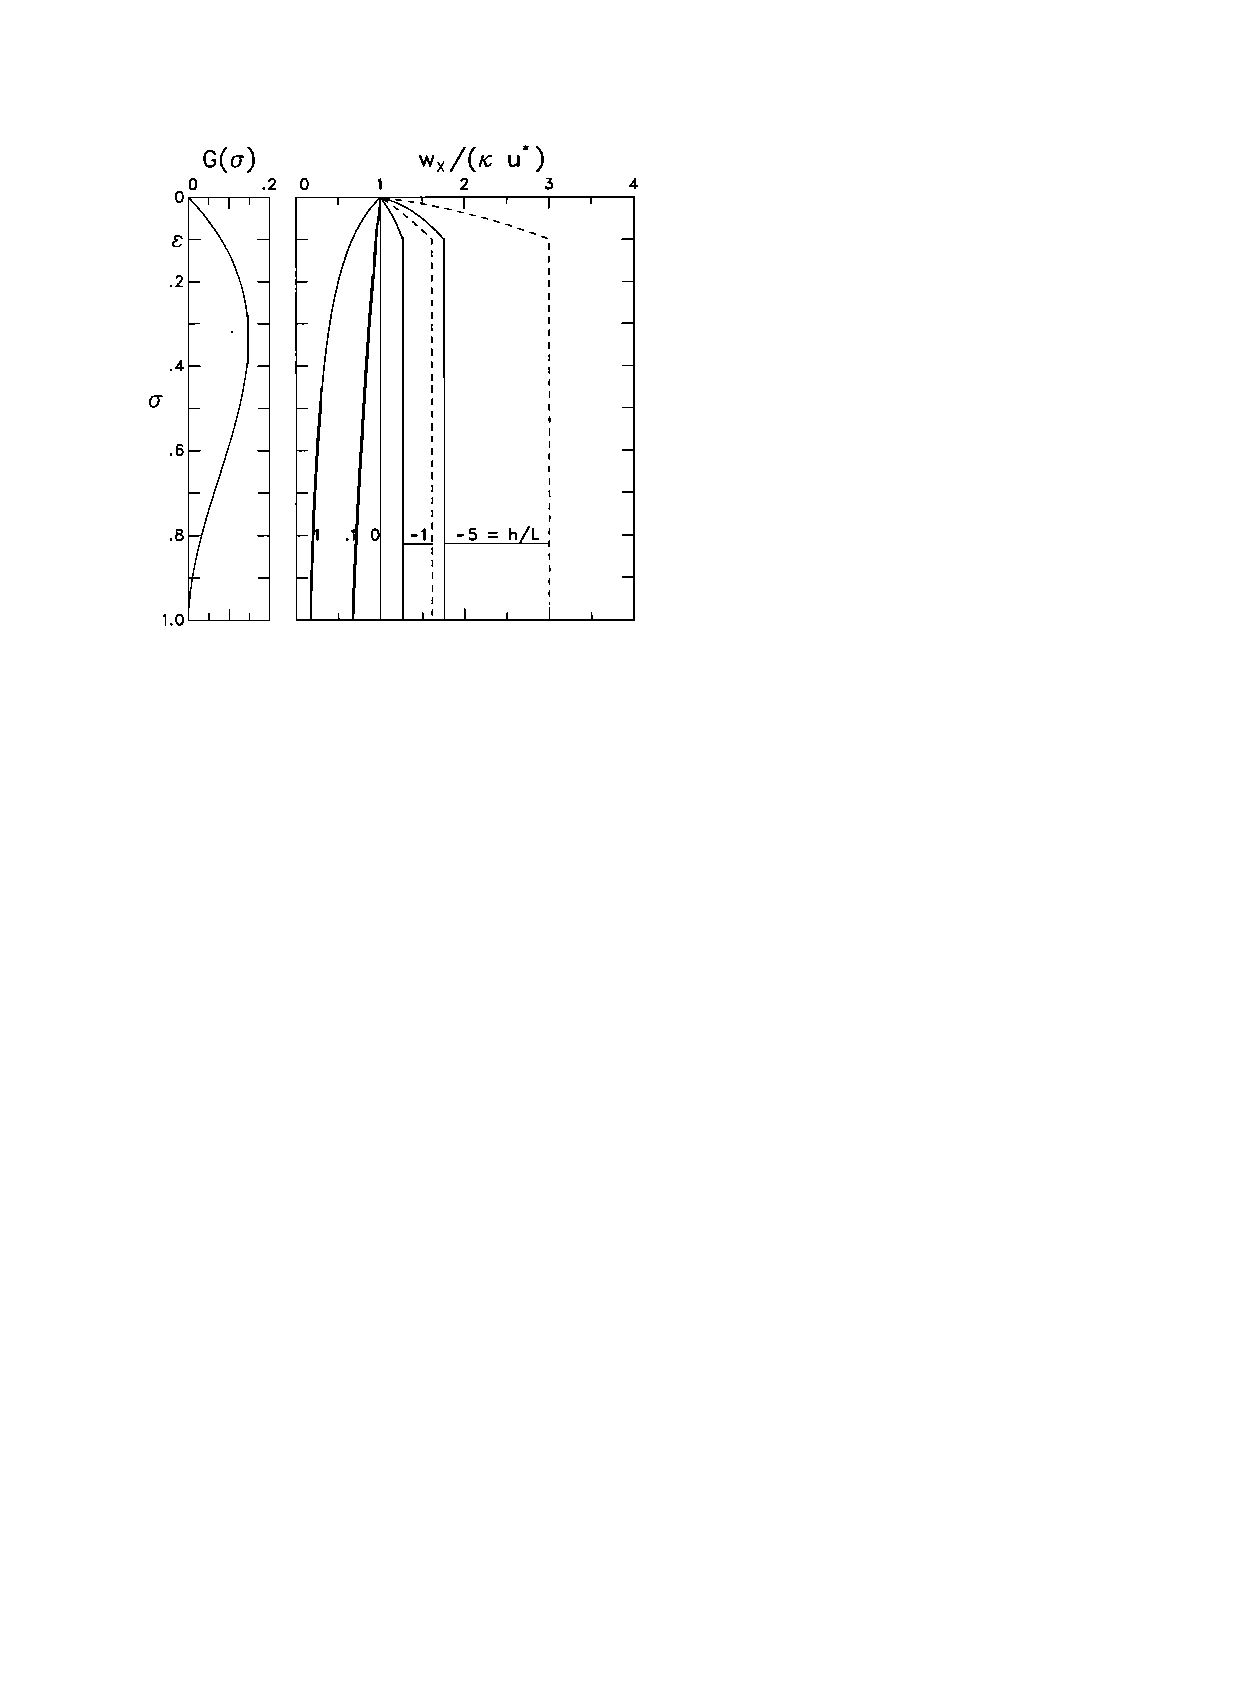
\includegraphics[angle=0,width=8cm]{./figs/LargeKPP_fig2.pdf}
\caption[Figure 2 from \cite{LargeKPP}]{ \sf This is a reproduction of
  Figure 2 from \cite{LargeKPP}.  The vertical axis is the
  dimensionless vertical coordinate $\sigma = d/h$ within the KPP
  boundary layer $0 \le \sigma \le 1$.  The left panel shows the
  vertical profile of the shape or structure function,
  $G_{\lambda}(\sigma)$, used to scale the vertical diffusivity via
  equation (\ref{eq:kpp-diffusivity-again}).  The analytic form shown
  here is given by $G_{\lambda}(\sigma) = \sigma \, (1-\sigma)^{2}$,
  which corresponds to the \cite{Troen_Mahrt1986} form and which is
  independent of the quantity $\Lambda$ being diffused.
  \cite{LargeKPP} chose a more general form, based on the need to
  match boundary layer diffusivities to interior diffusivities in
  which case the shape function becomes a function of $\lambda$.  We
  detail this approach in Section \ref{subsection:kpp-shape-function}.
  The right panel shows various examples of the normalized turbulent
  velocity scale $w_{\lambda}$ (called $w_{x}$ in \cite{LargeKPP}),
  with the examples differing by the value of the dimensionless ratio
  $h/L$ between the boundary layer depth, $h$, and the Monin-Obukhov
  length scale $L$.  For unstable buoyancy forcing, $L<0$, the
  velocity scale for scalars, $w_{s}$ (dashed lines), is greater than
  that for momentum, $w_{m}$ (solid lines).  For stable forcing,
  $L>0$, and both scalar and momentum have the same turbulent velocity
  scales, $w_{s} = w_{m}$.  In general, the turbulent velocity scale
  is enhanced with unstable surface buoyancy forcing, and reduced with
  stable buoyancy forcing.}
\label{fig:kpp-figure2-reproduced}
\end{center}
\rule{\textwidth}{0.005in}
\end{figure}
%%%%%%%%%%%%%%%%%%%%%%%%%%%%%%%%%%%%%%%%%%%%%%%%%%%%%%%%%%%%%%%%%%%%%%%%



\subsection{Similarity functions $\phi_{\Lambda}$}
\label{subsection:similarity-functions}

The vertical velocity scales are functions of the similarity functions
$\phi_{\Lambda}$, also called the dimensionless flux profiles.
Appendix B of \cite{LargeKPP} present analytic forms for these
functions, based on fits to available data, with their Figure B1
(reproduced here as Figure \ref{fig:large-etal-figureB1}) providing a
summary of the choices for the momentum function $\phi_{m}$ and the
scalar function $\phi_{s}$.  Both functions agree for stable buoyancy
forcing, and they depend linearly on the dimensionless Monin-Obukhov
length $\zeta = d/L = \sigma \, h/L$.


\subsubsection{The \cite{LargeKPP} choices for unstable buoyancy forcing}

For unstable buoyancy forcing, where $L<0$ and so $\zeta < 0$, there
are two regimes.  The scalar function $\phi_{s}$ is always less than
the momentum function $\phi_{m}$.  Hence, for unstable forcing there
is a larger turbulent velocity scale for the scalars than momentum,
and thus a larger vertical diffusivity for scalars.  The turbulent
Prandtl number, $Pr$, is given by the ratio of the flux functions
\begin{equation}
  \mbox{Pr} = K_{m} / K_{s} = w_{m} / w_{s} = \phi_{m} / \phi_{s}.
\label{eq:prandtl-number}
\end{equation}
The choices made by \cite{LargeKPP} lead to a Prandtl number in the
convective limit ($\zeta \rightarrow -\infty$) of 
\begin{equation}
 \mbox{Pr}  \rightarrow (c_{m}/c_{s})^{1/3} = 0.44,
\label{eq:convective-limit-prandtl}
\end{equation}
where $c_{m}$ and $c_{s}$ are parameters in the similarity functions
$\phi_{m}$ and $\phi_{s}$, respectively.

 
%%%%%%%%%%%%%%%%%%%% %%%%%%%%%%%%%%%%%%%%%%%%%
\begin{figure}[h!t]
\rule{\textwidth}{0.005in}
\begin{center}
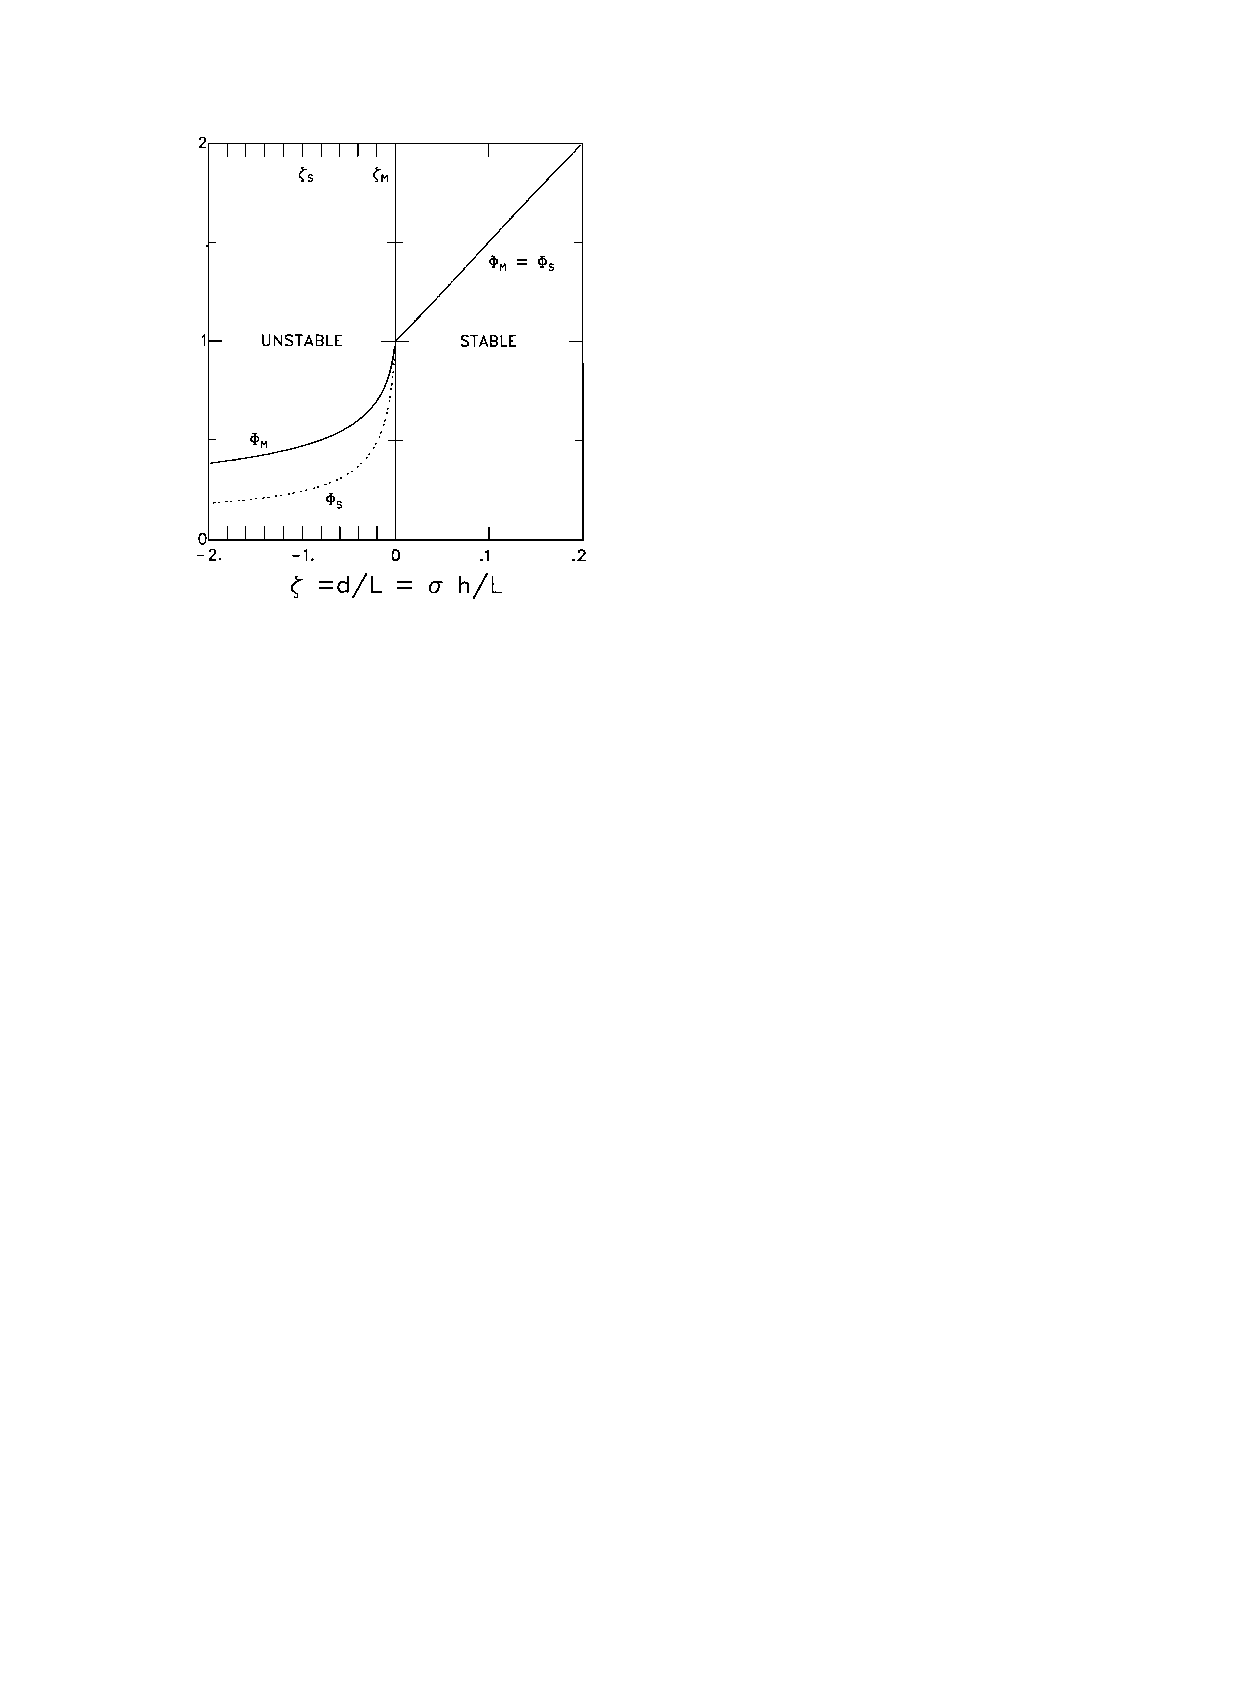
\includegraphics[angle=0,width=8cm]{./figs/LargeKPP_figB1.pdf}
\caption[Figure B1 from \cite{LargeKPP}]{\sf This is a reproduction of
  Figure B1 from \cite{LargeKPP}.  The vertical axis provides values
  for the dimensionless flux profiles, $\phi_{\Lambda}$, for momentum
  and scalars, and the horizontal axis gives the dimensionless
  Monin-Obukhov length scale $\zeta = d/L = \sigma \, h/L$.  There is
  a transition across the neutrally forced value of $\zeta = 0$.  For
  stable buoyancy forcing ($\zeta > 0$), both functions are the same,
  $\phi_{s} = \phi_{m}$, and are linear functions of $\zeta$. For
  unstable buoyancy forcing ($\zeta < 0$), the scalar function is less
  than momentum, $\phi_{s} < \phi_{m}$, with both functions falling
  off with a negative fractional power.  The analytic forms for the
  functions are given by equations (B1) and (B2) in \cite{LargeKPP}.}
\label{fig:large-etal-figureB1}
\end{center}
\rule{\textwidth}{0.005in}
\end{figure}
%%%%%%%%%%%%%%%%%%%%%%%%%%%%%%%%%%%%%%%%%%%%%%%%%%%%%%%%%%%%%%%%%%%%%%%%


\subsubsection{Alternative choices for unstable buoyancy forcing}

\cite{LargeKPP} chose two regimes for the unstable buoyancy forced
range, transitioning from different fractional exponents near $\zeta =
0$, to the same $-1/3$ power for larger negative $\zeta$.  The scalar
function $\phi_{s}$ falls off faster near $\zeta=0$, with a power
$-1/2$, whereas the momentum function $\phi_{m}$ falls off with a
$-1/4$ power.  This initial distinct fractional power falloff sets the
scale for the Prandtl number in this portion of $\zeta$ in the weakly
unstable regime.

Having two regimes for the negative buoyancy forcing adds complexity
to the algorithm.  We thus consider how well the original two-regime
forms for $\phi_{m}$ and $\phi_{s}$ can be fit using a single regime,
using only the fractional power $-1/3$.  Tests suggest that the
following forms may be suitable
\begin{equation}
   \phi_{m}(\zeta) = \left\{
 \begin{array}{lll}
  &1 + 5 \, \zeta      &\zeta > 0 \\
  &(1-9\zeta)^{-1/3}  &\zeta < 0 
 \end{array}
 \right.
\label{eq:phim-alternative}
\end{equation}
\begin{equation}
   \phi_{s}(\zeta) = \left\{
 \begin{array}{lll}
  &1 + 5 \, \zeta      &\zeta > 0 \\
  &(1-60\zeta)^{-1/3}  &\zeta < 0. 
 \end{array}
 \right.
\label{eq:phis-alternative}
\end{equation}
A comparison of the original forms from \cite{LargeKPP} to the
alternative forms is shown in Figure
\ref{fig:phi-alternative-kpp}. Also shown is the ratio of these two
functions which yields the turbulent Prandtl number according to
equation (\ref{eq:prandtl-number}).  The agreement between the
original forms and the new forms is worse when considering the Prandtl
number.  As discussed in the figure caption, a viable means for
simplifying the turbulent functions, without compromising much on the
values used in \cite{LargeKPP}, is to maintain original 3-region
$\phi_{s}$ form, but to simplify $\phi_{m}$ to 2-regions according to
equation (\ref{eq:phim-alternative}).


%%%%%%%%%%%%%%%%%%%% %%%%%%%%%%%%%%%%%%%%%%%%%
\begin{figure}[h!t]
\rule{\textwidth}{0.005in}
\begin{center}
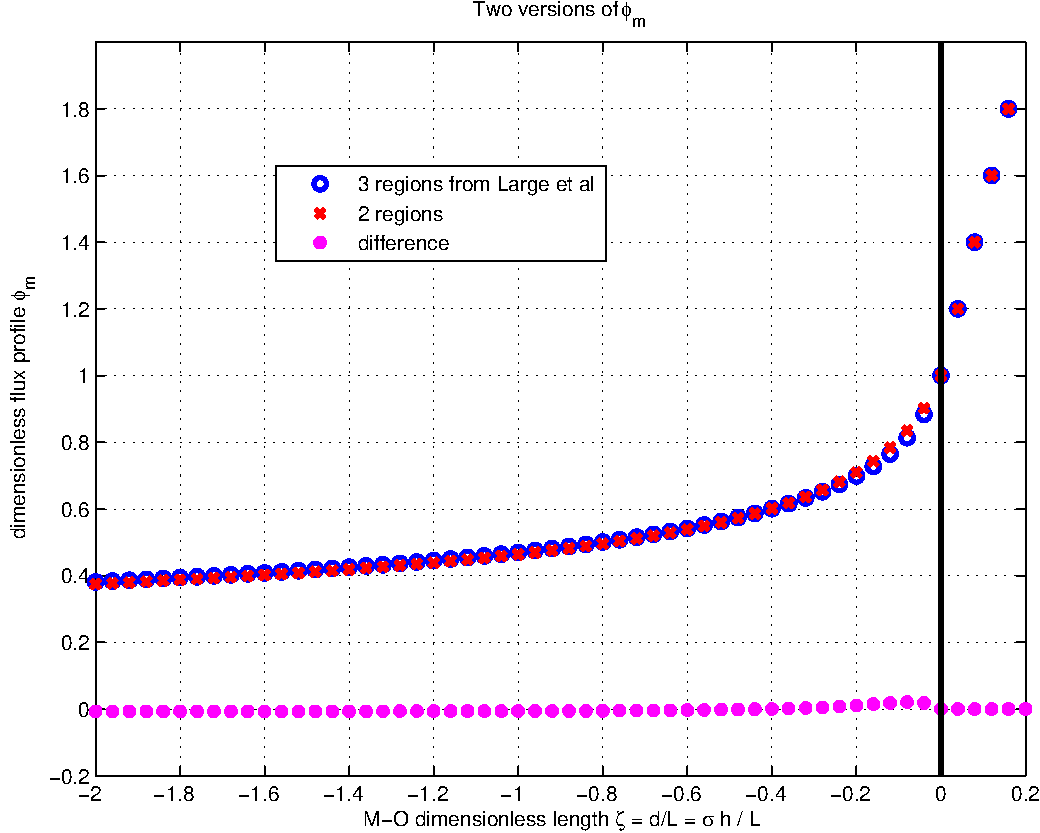
\includegraphics[angle=0,width=8cm]{./figs/phi_m_profiles.pdf}
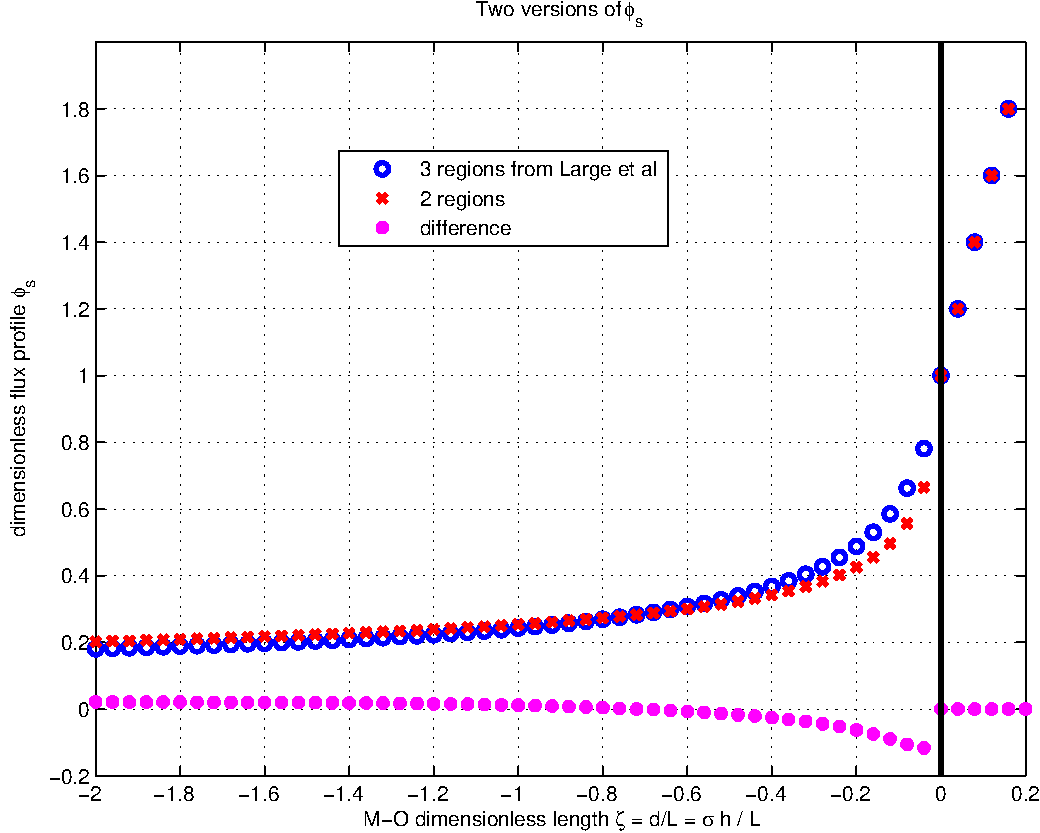
\includegraphics[angle=0,width=8cm]{./figs/phi_s_profiles.pdf}
\\
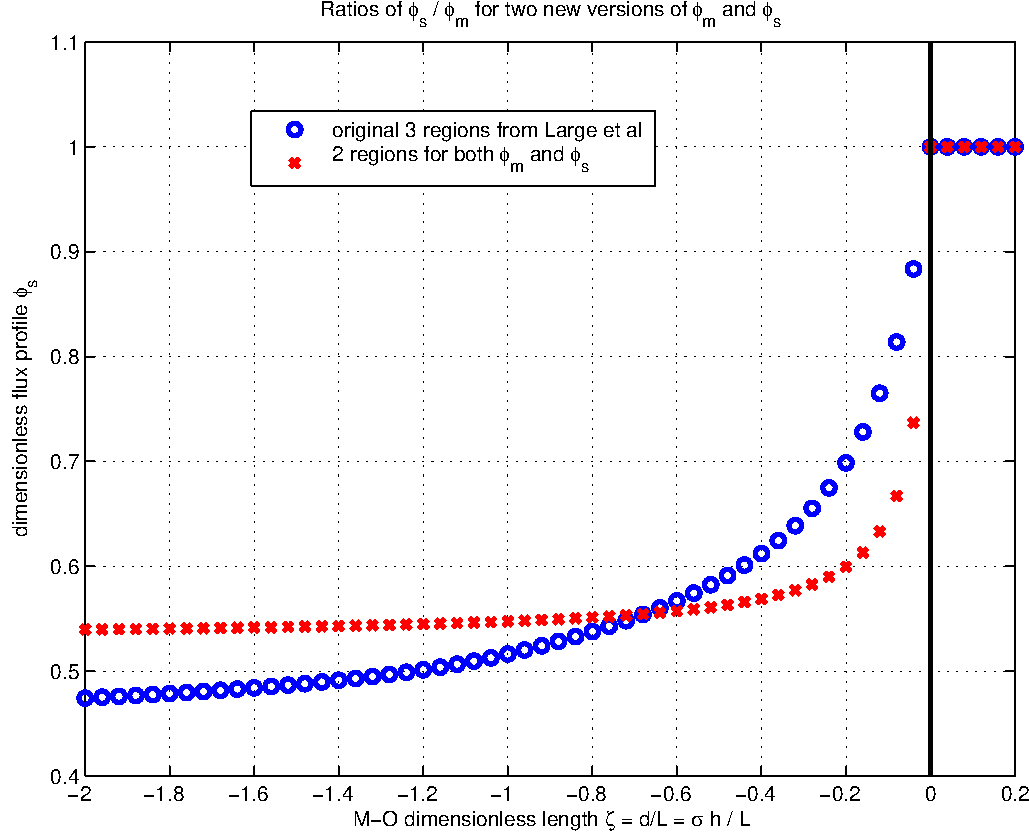
\includegraphics[angle=0,width=8cm]{./figs/prandtl_profiles_phim_phis.pdf}
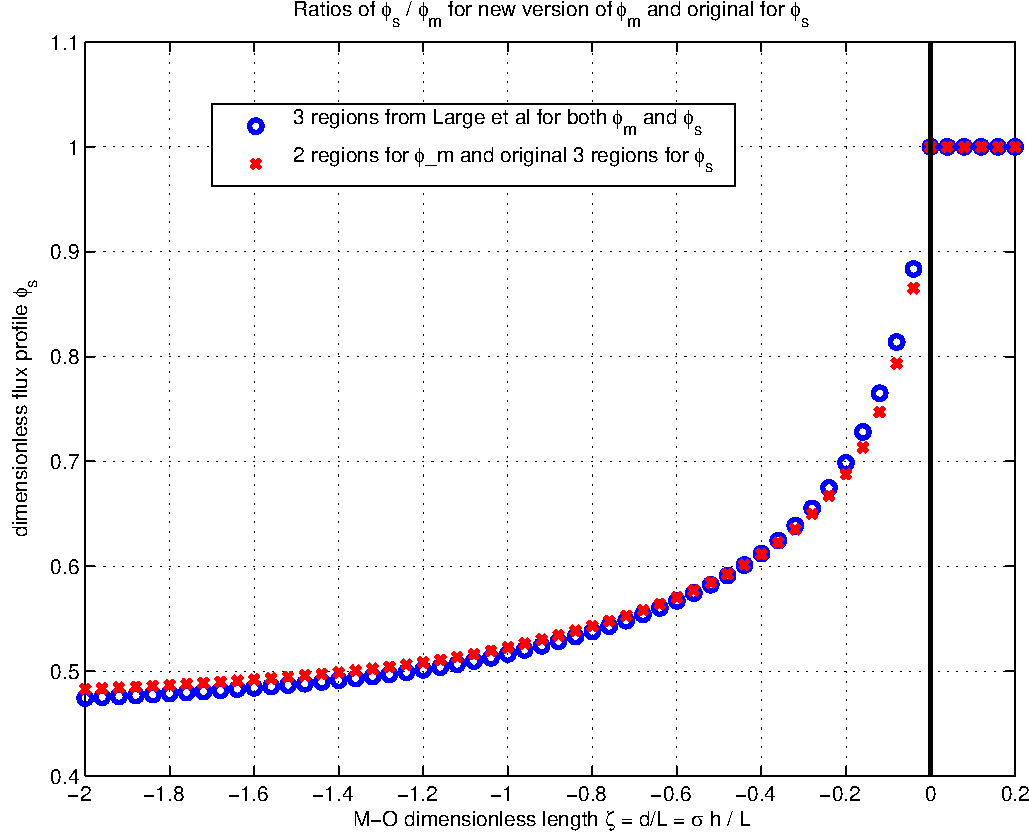
\includegraphics[angle=0,width=8cm]{./figs/prandtl_profiles_just_phim_new.pdf}
\caption[Alternative similarity functions]{\sf Shown here are 2-region
  flux profiles given by equations (\ref{eq:phim-alternative}) and
  (\ref{eq:phis-alternative}) as compared to the original 3-region
  profiles rom \cite{LargeKPP}.  We also show the ratio,
  $\phi_{s}/\phi_{m}$, which defines the turbulent Prandtl number or
  the ratio of the vertical momentum viscosity to vertical tracer
  diffusivity.  The top left panel shows the original 3-region
  $\phi_{m}$ as compared to the 2-region form
  (\ref{eq:phim-alternative}).  The agreement is quite close.  The top
  right panel shows the comparison for $\phi_{s}$, with the agreement
  not very good. The lower left panel shows the ratio
  $\phi_{s}/\phi_{m}$ for the original 3-region functions and the new
  2-region functions.  Their ratio amplifies the problems with the new
  $\phi_{s}$ form (\ref{eq:phis-alternative}).  The lower right panel
  shows the ratio of the original 3-region $\phi_{s}$ to the new
  2-region form of $\phi_{m}$.  These results suggest that to remain
  consistent with the original \cite{LargeKPP} results, it is feasible
  to switch to the 2-region form (\ref{eq:phim-alternative}) for
  $\phi_{m}$, but we must maintain the original 3-region form of
  $\phi_{s}$.}
\label{fig:phi-alternative-kpp}
\end{center}
\rule{\textwidth}{0.005in}
\end{figure}
%%%%%%%%%%%%%%%%%%%%%%%%%%%%%%%%%%%%%%%%%%%%%%%%%%%%%%%%%%%%%%%%%%%%%%%%


\subsection{The shape function $G_{\lambda}(\sigma)$}
\label{subsection:kpp-shape-function}

The vertical shape function $G_{\lambda}(\sigma)$ is given by the cubic
polynomial 
\begin{equation}
 G_{\lambda}(\sigma) = a_{0} + a_{1} \, \sigma + a_{2} \, \sigma^{2} + a_{3} \, \sigma^{3}.
\label{eq:structure-function-gsigma-again}
\end{equation}
As already noted when introducing this cubic expression (equation
(\ref{eq:structure-function-gsigma})), turbulent eddies do not cross
the ocean surface at $\sigma=0$, so the diffusivity should vanish at
$\sigma=0$.  This constraint is satisfied by setting
\begin{equation}
 a_{0} = 0.
\end{equation}
We now discuss further constraints to specify the remaining
coefficients.  

We start by rewriting the expression
(\ref{eq:specifying-structure-function}) that expresses the ratio of
turbulent fluxes within the surface layer to those at the surface
boundary 
\begin{equation}
  a_{1} + a_{2} \, \sigma = \left( \frac{ \overline{w \, \lambda}^{\sigma}}{\overline{w \, \lambda}^{\eta}} \right)
 \qquad  \mbox{surface layer: $0 \le \sigma \le \epsilon$.}
\label{eq:specifying-structure-function-again}
\end{equation}
Satisfying this relation at the ocean surface, $\sigma=0$, requires
\begin{equation}
 a_{1} = 1, 
\end{equation}
 so that 
\begin{equation}
  1 + a_{2} \, \sigma = \left( \frac{ \overline{w \, \lambda}^{\sigma}}{\overline{w \, \lambda}^{\eta}} \right)
 \qquad  \mbox{surface layer: $0 \le \sigma \le \epsilon$.}
\label{eq:specifying-structure-function-againB}
\end{equation}

Now define the ratio
\begin{equation}
  \beta_{\lambda} = \left( \frac{ \overline{w \, \lambda}^{\epsilon}}{\overline{w \, \lambda}^{\eta}} \right),
\label{eq:beta-lambda-defined}
\end{equation}
which is the ratio of the turbulent flux at the base of the surface
layer, $\sigma = \epsilon$, to the flux at the upper ocean interface,
$z=\eta$.  For atmospheric boundary layers, \cite{Troen_Mahrt1986} set
\begin{equation}
 \beta_{\lambda}  = 2 \, \epsilon \qquad \mbox{atmospheric boundary layers,} 
\end{equation}
with $\epsilon=0.1$.  \cite{Troen_Mahrt1986} further assume both the
shape function and its first derivative vanish at the base of the
boundary layer, $\sigma=1$.  These assumptions lead to the cubic
expression valid for all fluctuating fields $\lambda$
\begin{equation}
 G(\sigma) = \sigma \, (1-\sigma)^{2}   \qquad \mbox{atmospheric boundary layers,}
\end{equation}
with this function exhibited in the left panel of Figure
\ref{fig:kpp-figure2-reproduced}.  

\cite{LargeKPP} also assume the surface layer is 10\% of the boundary
layer, so that 
\begin{equation}
 \epsilon = 0.1 \qquad \mbox{KPP scheme.}
\end{equation}
However, they consider a more general approach for the remaining
approach to deriving the shape function.  The key reason to generalize
the atmospheric approach of \cite{Troen_Mahrt1986} is to admit the
possibility of ocean boundary layer turbulence to be impacted by
interior mixing, with this mixing parameterized by downgradient
vertical diffusion.  Such diffusion generally introduces distinct
diffusivities for tracers (e.g., double diffusion) as well as for
momentum (e.g., non-unit Prandtl number).  For these reasons,
\cite{LargeKPP} insist that both the diffusivity and its vertical
derivative match across the base of the boundary layer at $\sigma=1$.
This matching condition leads to the constraints (18) given by
\cite{LargeKPP}, which in turn leads to shape functions that are
dependent on the field being transported.

Matching both the shape function and its vertical derivative across
the boundary layer base adds complexity to the KPP algorithm.
Furthermore, it is unclear how accurate one can in fact satisfy both
matching conditions on a finite grid with potentially coarse vertical
grid spacing at the boundary layer base.  To simplify the KPP
algorithm, we drop the need to match the vertical derivative of the
diffusivity.  Instead, we assume continuity of the diffusivity with a
vanishing derivative at the boundary layer base, $\sigma=1$.  Setting
$\partial_{\sigma} G(\sigma) = 0$ at $\sigma=1$ leads to the relation
\begin{equation}
 3 \, a_{3} = -(1+ 2 \, a_{2}). 
\label{eq:a3-in-terms-of-a2}
\end{equation}
Matching diffusivities at $\sigma=1$ between the boundary layer and
interior value leads to
\begin{equation}
  a_{2}  = -2 + \left(\frac{3 \, K_{\lambda}(h)}{h \, w_{\lambda}(h)}
  \right),
\label{eq:a2-specified}
\end{equation}
where the diffusivity $K_{\lambda}(h)$ is determined by
parameterizations of interior mixing.  Substituting this expression
for $a_{2}$ into equation (\ref{eq:a3-in-terms-of-a2}) for $a_{3}$
leads to
\begin{equation}
 a_{3} = 1 - \left(\frac{2 \, K_{\lambda}(h)}{h \, w_{\lambda}(h)} \right).
\end{equation}
Allowing for the interior mixing to influence the KPP boundary layer
scheme suggests that the KPP calculation should be called {\it after}
the various methods used to compute interior diffusivities.  



\subsection{The non-local transport $\gamma_{\lambda}$}
\label{subsection:kpp-non-local-transport}

We now consider the parameterization for the non-local transport (see
Section \ref{subsection:kpp-nonlocal-transport-outline}) as suggested
by \cite{LargeKPP}.  Again, the KPP parameterization takes the form
(equation (\ref{eq:kpp-parameterization}))
\begin{equation}
  \overline{w \, \lambda} = -K_{\lambda} \left( \frac{\partial \Lambda}{\partial z} - \gamma_{\lambda} \right),
\label{eq:kpp-parameterization-yet-again}
\end{equation}
so that that non-local portion of the turbulent flux is parameterized
according to
\begin{equation}
 \overline{w \, \lambda}^{\mbox{\tiny non-local}} = K_{\lambda}  \, \gamma_{\lambda},  
\end{equation}
where $K_{\lambda}$ takes the form in equation
(\ref{eq:kpp-diffusivity-again}): 
\begin{equation}
 K_{\lambda}(\sigma) = h \, w_{\lambda}(\sigma) \, G_{\lambda}(\sigma).
\label{eq:kpp-diffusivity-yet-again}
\end{equation}
For completeness, we repeat elements of the outline presented in
Section \ref{subsection:kpp-nonlocal-transport-outline}.


\subsubsection{General features of $\gamma_{\lambda}$ with the KPP parameterization}

\begin{itemize}

\item \cite{Smyth_etal2002} consider a non-local term for momentum.
  Until their ideas have been fully tested in climate models, we
  follow recommendations from \citep{LargeKPP}, who set the non-local
  momentum transport to zero:
\begin{equation}
 \gamma_{\lambda} \; \; = \; \; 
\left\{
 \begin{array}{ll}
  0 \; \;  &\mbox{if $\lambda = (u,v,w)$ a velocity component}
 \\
  \ne 0 \; \; &\mbox{nonzero if $\lambda = \theta,s$ or another tracer.}
  \end{array}
 \right.
\end{equation}

  \item The non-local transport is non-zero only within the OBL:  
\begin{equation}
 \gamma_{\lambda} \; \; = \; \; 
  \left\{ 
  \begin{array}{ll}
   0 \; \; &\mbox{if $\sigma > 1$}
   \\ 
   \ne 0  \; \; &\mbox{if $0 \le \sigma \le 1$.}
  \end{array}
 \right.
\end{equation}

  \item The non-local transport is non-zero only in the presence of
    destabilizing negative surface ocean buoyancy flux:
\begin{equation}
 \gamma_{\lambda} \; \; = \; \; 
  \left\{ 
  \begin{array}{ll}
   0 \; \; &\mbox{for $B_{f} > 0$}
   \\ 
   \ne 0 \; \; &\mbox{for $B_{f} < 0$.}
  \end{array}
 \right.
\end{equation}


\item The non-local transport for temperature and arbitrary scalars is
  given by the following form for destabilizing negative surface ocean
  buoyancy fluxes:
\begin{align}
 \gamma_{\theta} &= 
   C_{s} \, \left( \frac{ \overline{w \, \theta}^{\eta} - Q_{R}/(\rho_{0} \, C_{p})  }{h \,  w_{\theta}(\sigma)}  
            \right) 
\label{eq:non-local-temp-kpp}
\\
 \gamma_{s} &= 
   C_{s} \, \left( \frac{ \overline{w \, s}^{\eta} }{h \,  w_{s}(\sigma)}  
            \right), 
\label{eq:non-local-scalar-kpp}
\end{align}
 where 
\begin{equation}
 C_{s} = C_{*} \, \kappa \, (c_{s} \, \kappa \, \epsilon)^{1/3},  
\label{eq:cs-and-cstar-defined}
\end{equation}
with 
\begin{equation}
 C_{*} = 10,
\label{eq:cstar-value-specified}
\end{equation}
and $Q_{R}$ is the heat flux from penetrative radiation given by
equation (\ref{eq:penetrative-heating-kpp}).

Combining the parameterizations (\ref{eq:non-local-temp-kpp}) and
(\ref{eq:non-local-scalar-kpp}) for the non-local term
$\gamma_{\lambda}$, with that for the vertical diffusivity
$K_{\lambda}$ in equation (\ref{eq:kpp-diffusivity-yet-again}) renders
the non-local flux parameterization in the form
\begin{align}
\overline{w \, \theta}^{\mbox{\tiny non-local}} &= K_{\theta}  \, \gamma_{\theta}
  = 
 G_{\lambda}(\sigma) \, C_{s} \, \left( \overline{w \, \theta}^{\eta} - Q_{R}/(\rho_{0} \, C_{p}) \right)
\label{eq:non-local-flux-kpp-param-temp}
\\
\overline{w \, s}^{\mbox{\tiny non-local}} &= K_{s}  \, \gamma_{s}
  = 
 G_{s}(\sigma) \, C_{s}\,\left( \overline{w \, s}^{\eta} \right).
\label{eq:non-local-flux-kpp-param-scalar}
\end{align}
Notice how explicit dependence on both the turbulent velocity scale,
$w_{\lambda}$, and boundary layer depth, $h$, drop out from the
parameterization of the non-local flux.

\end{itemize}



\subsubsection{Summary of the non-local transport parameterization} 

We now summarize the non-local transport for temperature and arbitrary
scalars, with \cite{LargeKPP} proposing a parameterization according
to the following expression, again valid just for destabilizing
negative surface ocean buoyancy fluxes (it vanishes for stable
buoyancy forcing):
\begin{align}
 \gamma_{\theta} &= 
   C_{s} \, \left( \frac{ \overline{w \, \theta}^{\eta} - Q_{R}/(\rho_{0} \, C_{\mbox{\tiny p}}^{o} )  }{h \,  w_{\theta}(\sigma)}  
            \right) 
\label{eq:non-local-temp-kpp-again}
\\
 \gamma_{s} &= 
   C_{s} \, \left( \frac{ \overline{w \, s}^{\eta} }{h \,  w_{s}(\sigma)}  
            \right).
\label{eq:non-local-scalar-kpp-again}
\end{align}
 In these expressions, we have 
\begin{equation}
 C_{s} = C_{*} \, \kappa \, (c_{s} \, \kappa \, \epsilon)^{1/3},  
\end{equation}
with \cite{LargeKPP} suggesting the value of 
\begin{equation}
 C_{*} = 10,
\end{equation}
whereas $C_{*} = 5$ in \cite{Smyth_etal2002}.  The von Karman constant
$\kappa = 0.40$ (equation (\ref{eq:von-karman-constant})) appears in
this expresion, as well as the fraction of the boundary layer assumed
to be occupied by the Monin-Obukhov surface layer
\begin{equation}
\epsilon = 0.1.
\end{equation}
The coefficient $c_{s}$ is set according to the similarity function
$\phi_{s}$ (Section \ref{subsection:similarity-functions}).

The flux $Q_{R}>0$ appearing in the $\gamma_{\theta}$ expression for
equation (\ref{eq:non-local-temp-kpp-again}) is the heat flux crossing
the ocean surface from shortwave radiation.  We split this penetrative
shortwave flux from the non-penetrative heat flux $\overline{w \,
  \theta}^{\eta}$, which is positive for cases where heat leaves the
ocean surface due to non-penetrative heat fluxes (i.e., longwave,
sensible, and latent).  The net heat flux crossing the ocean surface
is given by
\begin{equation}
 Q^{\mbox{\footnotesize heat}}= Q_{R} - \rho_{o} \, C_{\mbox{\tiny p}}^{o} \,  \overline{w \, \theta}^{\eta},
\label{eq:heat-flux-penetrative-and-non-penetrative}
\end{equation}
where $Q^{\mbox{\footnotesize heat}} > 0$ for heat entering the ocean.
The parameterized non-local transport term thus takes the following
form for temperature
\begin{equation}
 \gamma_{\theta} = -\left(\frac{ C_{s}}{\rho_{o}  \, C_{\mbox{\tiny p}}^{o} } \right) 
  \frac{ Q^{\mbox{\footnotesize heat}} }{h \,  w_{\theta}(\sigma)}.  
\label{eq:non-local-temp-kpp-again-again}
\end{equation}
Generally the negative buoyancy forcing that gives rise to the
non-local transport is associated with cooling
($Q^{\mbox{\footnotesize heat}} < 0$), so that 
\begin{equation}
  \gamma_{\theta} > 0 \qquad \mbox{surface cooling}.
\label{eq:surface-cooling-gamma-theta}
\end{equation}

Combining the parameterizations
(\ref{eq:non-local-temp-kpp-again-again}) and
(\ref{eq:non-local-scalar-kpp-again}) for the non-local term
$\gamma_{\lambda}$, with that for the vertical diffusivity
$K_{\lambda}$ in equation (\ref{eq:kpp-diffusivity}) renders the
non-local flux parameterization in the form
\begin{mdframed}[backgroundcolor=lightgray!50]
\begin{align}
\overline{w \, \theta}^{\mbox{\tiny non-local}} &= K_{\theta}  \, \gamma_{\theta}
  = 
 - G_{\theta}(\sigma) \, C_{s} \, \left( \frac{ Q^{\mbox{\footnotesize heat}}}{ \rho_{o}  \, C_{\mbox{\tiny p}}^{o} } \right)
\label{eq:non-local-flux-kpp-param-temp-again}
\\
\overline{w \, s}^{\mbox{\tiny non-local}} &= K_{s}  \, \gamma_{s}
  = 
 G_{s}(\sigma) \, C_{s}\,\left( \overline{w \, s}^{\eta} \right).
\label{eq:non-local-flux-kpp-param-scalar-again}
\end{align}
\end{mdframed}
Notice how explicit dependence on both the turbulent velocity scale,
$w_{\lambda}$, and boundary layer depth, $h$, drop out from the
parameterization of the non-local flux.



\subsubsection{Potential problems with the parameterized non-local transport}

Experience has shown that there are cases when the parameteried
non-local flux, (\ref{eq:non-local-flux-kpp-param-temp}) of
(\ref{eq:non-local-flux-kpp-param-scalar}), can produce values larger
than the surface flux.  That is, one may realize cases when 
\begin{equation}
   G_{\lambda}(\sigma) \, C_{s} > 1 \qquad \mbox{non-local flux greater than surface flux.}
\end{equation}
This situation arises particularly near the boundary layer base,
$\sigma=1$, when the interior diffusivity is large.  The matching
conditions employed by \cite{LargeKPP} (Section
\ref{subsection:kpp-shape-function}) then lead to a very large value
for the shape function $G(\sigma)$.  In this case, one may be exposed
to the production of extrema in the tracer field.  In the presence of
sea-ice, problems may arise particularly in fresh water regions such
as the Baltic Sea where the thermal expansion coefficient is negative,
$\alpha < 0$ (Martin Schmidt, personal communication).

The following modifications to the original \cite{LargeKPP} scheme
have been found useful to reduce the potential for the non-local term
to be problematic. 
\begin{itemize}

\item {\sc interior gravitational instabilities}: When the vertical
 stratification is unstable ($N^{2} < 0$), vertical diffusivity is
  enhanced to remove the gravitational instability. Notably, it is
  {\it not} appropriate to enhance the diffusivity within the KPP
  boundary layer, beyond that already computed via the KPP scheme,
  even when $N^{2} < 0$.  On those occasions when the instabilities
  appear beneath the boundary layer, diffusivities are enhanced.  If
  one insisted that such diffusivities should match those in the
  boundary layer, then the shape function $G(\sigma)$ would indeed
  become quite large in magnitude.  Hence, NCAR recommends that one
  pull the ``convective adjustment'' portion of the mixing scheme
  outside of the KPP portion of the algorithm.  That is, the interior
  convective instability diffusivities are {\it not} matched to the
  KPP boundary layer diffusivities.  

\item {\sc simpler matching}: As noted in Section
  \ref{subsection:kpp-shape-function}, we propose to simplify the
  matching at the boundary layer base, so that only the diffusivities
  match across the boundary layer base, rather than also insisting on
  the derivative of the diffusivities as proposed by \cite{LargeKPP}.
  The simplified matching condition leads to less problems computing
  discrete vertical derivatives of the diffusivities, and in turn
  produces more well regularized diffusivities and shape functions.

\end{itemize}


\subsection{Bulk Richardson number and the OBL thickness}
\label{subsection:kpp-obl-thickness}

\cite{LargeKPP} define the KPP boundary layer depth to be an
interpolation to the depth at which the bulk Richardson number,
$\mbox{Ri}_{b}$, equals to a critical Richardson number,
\begin{equation}
 \mbox{Ri}_{c}  = \mbox{critical bulk Richardson number}. 
\label{eq:critical-bulk-richardson-number}
\end{equation}
Smaller values for $\mbox{Ri}_{b}$, including negative values, signal
that we are still in the boundary layer, whereas larger values are
beneath.  The critical value $\mbox{Ri}_{c}$ sets a threshold for
upper ocean mixing, with such enabling behaviour that is sensitive to
its precise value.

The bulk Richardson number is a non-local version of the gradient
Richardson number defined in Section
\ref{section:gradient-richardson-number-elements}.  It aims to measure
the ability of an upper ocean eddy, with buoyancy set by values of
temperature and salinity in the surface layer (Figure
\ref{fig:boundary-layer-schematic-kpp}), to move downward in the water
column, overcoming the resistence from stratification and aided by
both resolved and unresolved vertical shear.  Presumably at some
point, such boundary layer eddies will be suppressed by the reduced
shear and increased buoyancy stratification present below the boundary
layer.

Using the notation from \cite{LargeKPP}, we may write the bulk
Richardson number at a distance $d$ from the ocean surface in the form
\begin{equation}
  \mbox{Ri}_{b}(d) = \frac{d \, [B_{r} - B(d) ]}{ |{\bf U}_{r} - {\bf U}(d)|^{2} + U_{t}^{2}}. 
\label{eq:bulk-ri-large-kpp-large-etal-form}
\end{equation}
This calculation makes use of the surface layer averaged buoyancy,
$B_{r}$, and surface layer averaged horizontal velocity, ${\bf
  U}_{r}$, where the surface layer is defined by $0 \le \sigma \le
\epsilon$ (Figure \ref{fig:boundary-layer-schematic-kpp}). The term
$U_{t}^{2}$ is associated with parameterized unresolved vertical
shears that may act to further reduce the bulk Richardson number.

Using notation introduced in the local gravitational stability
calculation from Section \ref{section:buoyancy-frequency-elements}, we
write the bulk Richardson number in the form
\begin{equation}
  \mbox{Ri}_{b}(d) = \left( \frac{d \, g}{\rho_{o}} \right) 
   \left( 
   \frac{\rho[\Theta(d), S(d), p(d)]   - \rho[\Theta_{r}, S_{r}, p(d)]}{ |{\bf U}_{r} - {\bf U}(d)|^{2} + U_{t}^{2}}
  \right). 
\label{eq:bulk-ri-large-kpp}
\end{equation}
The density $\rho[\Theta(d), S(d), p(d)]$ is the {\it in situ} value
at a distance $d$ from the surface.  The density $\rho[\Theta_{r},
S_{r}, p(d)]$ is based on an adiabatic and isohaline displacement from
the surface layer to the depth $d$.  Now consider three cases to
expose the physics of the bulk Richardson number.
\begin{itemize}

\item {\sc Surface eddy has negative relative buoyancy}: If the
  density $\rho[\Theta_{r}, S_{r}, p(d)]$ is greater than the {\it in
    situ} density, $\rho[\Theta(d), S(d), p(d)]$, then a surface layer
  parcel can move downwards and the boundary layer based has yet to be
  reached.  That is, the surface layer parcel has negative buoyancy
  relative to the ambient fluid.  This situation leads to a negative
  bulk Richardson number, in which case the criteria $\mbox{Ri}_{b}(d)
  > \mbox{Ri}_{c}$ has not yet been reached.

\item {\sc Surface eddy has positive relative buoyancy and ambient
    fluid has strong shears}: If the density $\rho[\Theta_{r}, S_{r},
  p(d)]$ is less than the {\it in situ} density, a surface layer eddy
  has positive buoyancy relative to the ambient fluid.  However, if
  the vertical shear is large, then the bulk Richardson number can
  still be less than the critical value, in which case mechanically
  induced mixing is still large and the boundary layer base has yet to
  be reached.

\item {\sc Surface eddy has positive relative buoyancy and ambient
    fluid has weak shears}: Finally, if a surface eddy has positive
  relative buoyancy and the ambient fluid has weak shears, then at
  some point the bulk Richardson number will become larger than the
  critical value.  Interpolating to where that cross-over occurs
  determines the boundary layer thickness $h$.  

\end{itemize}


\subsubsection{Non-local gravitational stability}

Section \ref{section:buoyancy-frequency-elements} presents a general
discussion of local gravitational stability.  Much of that material is
useful for the purpose of determining gravitational stability for
parcels that are a finite distance from one another.  However, there
is one aspect of the discussion in Section
\ref{section:buoyancy-frequency-elements} that differs from the
present considerations.  Namely, we are here always considering
downward displacements of parcels from the surface layer.  The reason
is that we are concerned with parcels starting from the surface layer
moving downwards in an adiabatic and isohaline manner, with the
difficulty of such motion determined by the ambient stratification and
shear.  Figure \ref{fig:cvmix_stability_nonlocal} illustrates this
situation.  We are not interested in the complement movement of a deep
parcel towards the surface.


%%%%%%%%%%%%%%%%%%%% %%%%%%%%%%%%%%%%%%%%%%%%%
\begin{figure}[h!t]
\rule{\textwidth}{0.005in}
\begin{center}
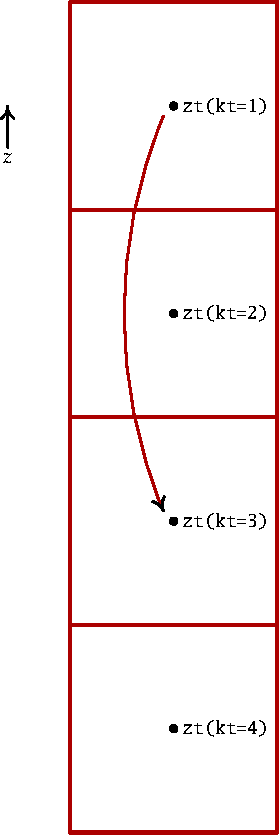
\includegraphics[angle=0,width=3cm]{./mfpic_figs/cvmix_stability_nonlocal.pdf}
\caption[Determining non-local gravitational stability]{\sf Schematic
  of the adiabatic and isohaline parcel displacement that is used to
  determine non-local gravitational stability for computing the bulk
  Richardson number according to equation
  (\ref{eq:bulk-ri-large-kpp}).  The reference temperature and
  salinity of this displaced parcel is set according to values
  determined in the surface layer, here approximated by the value at
  the top model grid cell with vertical position {\tt zt(kt=1)}.  The
  density of this parcel is then computed using the surface layer
  temperature and salinity and the local {\it in situ} pressure.  This
  displaced parcel's density is then compared to the ambient {\it in
    situ} density using the local temperature, salinity, and pressure.
  We illustrate that process by displacing the parcel to {\tt
    zt(kt=3)}.  If the resulting bulk Richardson number is larger than
  the critical value, the base of the KPP boundary layer is at or
  shallower than {\tt zt(kt=3)}, with interpolation used to determine
  the KPP boundary layer thickness $h$.  If the bulk Richarson number
  is less than the critical value, the boundary layer bottom has yet
  to be reached, so the downward search continues.}
\label{fig:cvmix_stability_nonlocal}
\end{center}
\rule{\textwidth}{0.005in}
\end{figure}
%%%%%%%%%%%%%%%%%%%%%%%%%%%%%%%%%%%%%%%%%%%%%%%%%%%%%%%%%%%%%%%%%%%%%%%%

The expression (\ref{eq:bulk-ri-large-kpp}) presents a direct means
for computing the non-local gravitational stability via the
computation of the density difference, written here using discrete
notation from Figure  \ref{fig:cvmix_stability_nonlocal}
\begin{equation}
 \delta\rho[{\tt kt},r]  = \rho[\Theta({\tt kt}), S({\tt kt}), p({\tt kt} ]  -\rho[\Theta_{r}, S_{r}, p({\tt kt})],
\label{eq:delta-density-for-nonlocal-stability}
\end{equation}
where the surface layer values $\Theta_{r}, S_{r}$ are typically
approximated by the values as {\tt kt =1}.  This approximation breaks
down for stable boundary layers with vertical grid spacing finer than
roughly 2~m, in which case an averaging is required.

There is an alternative method to approximate $\delta\rho[{\tt kt},r]$
based on linear truncations of Taylor series expansions.  The
alternative leads to a sum of squared buoyancy frequencies, analogous
to the expression
(\ref{eq:infinitesimal-delta-rho-elements-downward}).  There are some
advantages offered by the alternative approach, namely there are fewer
calculations of the equation of state, assuming we already have the
expansion coefficients $\alpha$ and $\beta$.  However, the deeper the
boundary layer, and the more nonlinear the equation of state, the less
accurate the approximation becomes.  We therefore recommend the more
exact calculation based on the density differences in equation
(\ref{eq:delta-density-for-nonlocal-stability}).

For completeness, we develop the alternative approach.  For this
purpose, consider a displacement from level {\tt kt = 1} to {\tt kt
  >1}, in which we need to compute $\rho[\Theta({\tt kt=1}),S({\tt
  kt=1}),p({\tt kt>1})]$.  Truncating a Taylor series at leading order
yields
\begin{equation}
 \rho[\Theta(1),S(1),p({\tt kt>1})]
 \approx 
 \rho[\Theta(1),S(1),p(1)] 
 - \sum\limits_{{\tt n  = 1}}^{{\tt kt}}
   {\tt dzw(n+1)} \,  \left( \frac{\partial \rho}{\partial p} \, \frac{\partial p}{\partial z}
   \right)_{ {\tt zt(n)} }.
\end{equation}
A similar expression for the {\it in situ} density $\rho[\Theta({\tt
  kt}), S({\tt kt}), p({\tt kt} ]$
\begin{equation}
 \rho[\Theta({\tt kt}),S({\tt kt}),p({\tt kt})]
 \approx 
 \rho[\Theta(1),S(1),p(1)] 
 - \sum\limits_{{\tt n  = 1}}^{{\tt kt}}
   {\tt dzw(n+1)} \,  \left( 
   \frac{\partial \rho}{\partial p} \, \frac{\partial p}{\partial z}
   + 
  \frac{\partial \rho}{\partial \Theta} \, \frac{\partial \Theta}{\partial z}
  +
  \frac{\partial \rho}{\partial S} \, \frac{\partial S}{\partial z}
   \right)_{ {\tt zt(n)} }.
\end{equation}
These results lead to the approximation 
\begin{equation}
\begin{split}
 \delta\rho[{\tt kt},r]  &= \rho[\Theta({\tt kt}), S({\tt kt}), p({\tt kt} ]  -\rho[\Theta_{r}, S_{r}, p({\tt kt})]
 \\
 &\approx 
 -\sum\limits_{{\tt n  = 1}}^{{\tt kt}}
   {\tt dzw(n+1)} \,  \left( 
 \frac{\partial \rho}{\partial \Theta} \, \frac{\partial \Theta}{\partial z}
  +
  \frac{\partial \rho}{\partial S} \, \frac{\partial S}{\partial z}
   \right)_{ {\tt zt(n)} }
\\
 &=
 \sum\limits_{{\tt n  = 1}}^{{\tt kt}}
   {\tt dzw(n+1)} \,  \left( 
 \rho \, \alpha \, \frac{\partial \Theta}{\partial z}
  -
  \rho \, \beta \, \frac{\partial S}{\partial z}
   \right)_{ {\tt zt(n)} }
\\
 &= 
 \frac{1}{g} 
  \sum\limits_{{\tt n  = 1}}^{{\tt kt}}
   {\tt dzw(n+1)} \,  \left( \rho \, N^{2} \right)_{ {\tt zt(n)} }.
\end{split}
\label{eq:summed-n2-for-nonlocal-stability}
\end{equation}
Again, this result is analogous to the approximate forms given in
Section \ref{subsection:buoyancy-frequency-and-stability} for the
local calculation of gravitational stability.  However, for both the
local and non-local calculation of stability, we recommend the more
exact approach that does not perform a trunction, particularly in
regions of deep mixing in the high latitudes. Making the approximation
may also compromise the ability of the KPP scheme to include
thermobaric convection.  We are thus reticent to recommend this
approach, and instead prefer the original approach given by equation
(\ref{eq:bulk-ri-large-kpp}).


\subsubsection{Unresolved shear $U_{t}$}
\label{subsubsection:unresolved-shear}

The shear, $U_{t}/d$, in the bulk Richardson number
(\ref{eq:bulk-ri-large-kpp}) acknowledges the potential presence of
unresolved shears that can impact on the boundary layer depth.
\cite{LargeKPP} present an argument on page 372 that focuses on an
unresolved shear that reduces to a desired form for the case of pure
convection
\begin{equation}
 U_{t}^{2}(d) = d \, \left( \frac{C_{v} \,  (-\beta_{T})^{1/2}}{\mbox{Ri}_{c} \, \kappa^{2}} \right)
  (c_{s} \, \epsilon)^{-1/2} \, N \; w_{s}.
\label{eq:unresolved-shear-kpp}
\end{equation}
 The constant $C_{v}$ sets the buoyancy frequency at the entrainment
 depth, and its value is expected to be 
\begin{equation}
 1 < C_{v} < 2. 
\label{eq:Cv-values-given} 
\end{equation}
The constant $c_{s}$ is part of the similarity functions discussed in
Section \ref{subsection:m-o-similarity-functions}.  The constant
$\beta_{T}$ is discussed in the caption to Figure
\ref{fig:kpp-figure1-reproduced}, and is represents the ratio of the
buoyancy flux at the entrainment depth, $h_{e}$, to the buoyancy flux
at the surface,
\begin{equation}
 \overline{w \, b}^{d=h_{e}} = \beta_{T}   \; \overline{w \, b}^{d=0},
\end{equation}
 with 
\begin{equation}
 \beta_{T} \approx -0.2
\end{equation}
an empirical result.  The critical Richardson number, $\mbox{Ri}_{c}$, is
used to determine when the boundary layer base is reached, in which
case stratification and/or reduced shear lead to a bulk Richardson
number larger than the critical value.  \cite{LargeKPP} choose the
value
\begin{equation}
 \mbox{Ri}_{c} = 0.3.  
\label{eq:large-critical-bulk-ri}
\end{equation}
The dimensionless number $\epsilon$ determines the thickness of the
surface layer as in Figure \ref{fig:boundary-layer-schematic-kpp},
with 
\begin{equation}
 \epsilon = 0.1 
\end{equation}
 chosen by \cite{LargeKPP}. 

It is notable that there are no surface gravity wave parameters in the
specification of the unresolved shear.  We have more to say on this
topic in Section \ref{section:surface-waves-and-kpp}. 


\subsubsection{Restrictions on $h$ under stable buoyancy forcing}

\cite{LargeKPP} suggest on page 372 that for stable buoyancy forcing,
$B_{f} > 0$, the boundary layer thickness, $h$, should be no larger
than either the Monin-Obukhov length scale, $L$, or the Ekman
length scale, 
\begin{equation}
 h_{E} = 0.7 \; u_{*} /|f|,
\label{eq:ekman-thickness}
\end{equation} 
with $f$ the Coriolis parameter.  The following reasons are noted to
motivate these two restrictions.
\begin{itemize}
\item {\sc Monin-Obukhov}: At depths deeper than $L$, buoyancy
  stratification suppresses the mechanically forced turbulence, thus
  cutting off the boundary layer.

  \item {\sc Ekman}: The Ekman depth is the extent of the boundary
    layer in neutral stratification ($N^{2} = 0$).  With stable
    buoyancy forcing, $B_{f} > 0$, we then expect the boundary layer
    depth to be less than the Ekman depth.  Note that \cite{LargeKPP}
    do not mention the origin of the $0.7$ factor in equation
    (\ref{eq:ekman-thickness}).

\end{itemize}

As noted in \cite{LargeKPP} and \cite{Large_Gent1999}, the restriction
on boundary layer thickness based on the Monin-Obukhov length has been
dropped in the NCAR implementation of KPP, as it does not lead to
favorable effects.  Dropping this constraint is also supported by the
results from \cite{Shchepetkin2005} and \cite{Lemarie_etal2012a}.
Likewise, the constraint based on the Ekman depth is not used at NCAR,
as little sensitivity was seen with its use.  Hence, there are no
restrictions for the maximum boundary layer depth under stable forcing
imposed by the NCAR implementation of KPP.  Such is the standard
approach used in the CVMix implementation.

The key problem with the Monin-Obukhov length scale, $L$, relates to
the question of how to include penetrative shortwave heating in the
calculation of the buoyancy forcing, $B_{f}$ (Section
\ref{subsection:buoyancy-forcing-obl}).  Depending on the depth over
which the penetrative heating is included (equation
(\ref{eq:penetrative-buoyancy-kpp})), one can produce a positive
Monin-Obukhov length (if including sufficient shortwave heating) or
negative (if including less heating). Since there is no fundamental
reason to choose a particular amount of the shortwave when considering
the total buoyancy forcing, there is no compelling reason to enforce
the $L$ constraint on boundary layer thickness.


\subsubsection{Noise in the boundary layer thickness}

Experience in MOM, POP, and ROMS indicate that the KPP boundary layer
thickness, $h$, can become quite noisy.  Noise in the boundary layer
thickness can translate into noise in the tracer fields within the
boundary layer.  Hence, it is common practice to apply a horizontal
smoothing operator, such as a Laplacian, to $h$ prior to its use in
computing the diffusivity or non-local transport.

The horizontal smoothing of $h$ poses an algorithmic problem for
CVMix, since CVMix modules ideally know nothing about the horizontal
grid.  There are two possible options that may be considered.
\begin{itemize}

\item {\sc intermediate $h$ sent back to calling model}: One option is
  to compute $h$ in CVMix; send it immediately back to the
  calling model for smoothing; then have the smoothed $h$ used for
  further KPP computations such as the diffusivity and non-local
  term.  

\item {\sc use previous $h$}: We compute the new value of $h$ within a
  particular call to the CMVix-KPP module, and we send this unsmoothed
  $h$ back to the calling model at the end of the CVMix-KPP module.
  But for computing the KPP diffusivities and non-local term within
  CVMix, we use the previous time step value $h$, with this earlier $h$
  having been smoothed by the calling model.  This approach requires
  storing $h$ in restart files, but that is easily handled by the
  calling model.  

\end{itemize}



\subsection{Surface boundary condition}
\label{subsection:kpp-surface-boundary-condition}

The parameterized non-local turbulent flux satisfies a no-flux
boundary condition at the ocean surface, so that
\begin{equation}
  \overline{w \, \lambda}^{\mbox{\tiny non-local}} = K_{\lambda} \;  \gamma_{\lambda}  = 0 \qquad \mbox{at $z=\eta$}.
\label{eq:non-local-surface-bc}
\end{equation}
This boundary condition is satisfied by ensuring that the
non-dimensional vertical shape function $G(\sigma)$ vanishes at
$\sigma = 0$, which means that
\begin{equation}
   K_{\lambda}  = 0   \qquad \mbox{at $z=\eta$}.
\end{equation}
We also set the local closure portion of the flux to zero at the
surface
\begin{equation}
\overline{w \, \lambda}^{\mbox{\tiny local}} = -K_{\lambda} \left( \frac{\partial \Lambda}{\partial z} \right) = 
 0  \qquad \mbox{at $z=\eta$},
\label{eq:no-flux-local}
\end{equation}
which again follows since $K_{\lambda} = 0$ at $z=\eta$.  However, to
incorporate the non-advective surface boundary fluxes (e.g.,
shortwave, longwave, latent, and sensible heat fluxes), we we follow
the usual convention these fluxes enter through the vertical diffusion
equation surface flux boundary condition, so that in effect we have
\begin{equation}
\overline{w \, \lambda}^{\eta}  = Q^{\lambda}  \qquad \mbox{at $z=\eta$}. 
\label{eq:surface-boundary-flux}
\end{equation}


\subsection{Convergence into a surface grid cell}
\label{subsection:kpp-surface-cell-tendency}

At the surface boundary, the parameterized local and non-local flux
components vanish.  However, these flux components are generally quite
large at the bottom interface of the $k=1$ cell.  Hence, there is a
sizable convergence of the parameterized fluxes into the $k=1$ cell.
We can furthermore account for the predominance of a tendency for the
parameterized local fluxes to cool the $k=1$ cell, whereas the
parameterized non-local fluxes generally warm this cell.

In a region stably stratified in temperature, we have temperature
increasing upwards in the column, $\partial \Theta / \partial z >
0$. Assuming such stratification for the upper ocean, the downgradient
diffusive flux
\begin{equation}
\overline{w \, \theta}^{\mbox{\tiny local}} = -K_{\theta} \left( \frac{\partial \Theta}{\partial z} \right) < 0,
\end{equation}
is then negative at the lower face of the $k=1$ cell.  With the
no-flux boundary condition (\ref{eq:no-flux-local}) at the ocean
surface, the parameterized local diffusive flux will thus cool the top
model grid cell. For $k > 1$ interior cells, the diffusive flux either
cools or warms, depending on curvature in the temperature field.

The non-local transport is non-zero only for cases of negative
buoyancy forcing.  Assuming such forcing occurs due to a cooling
surface heat flux, we already showed in Section
\ref{subsection:kpp-surface-boundary-condition} that $\gamma_{\theta}
> 0$ for cooling (equation (\ref{eq:surface-cooling-gamma-theta})).
With the no-flux surface boundary condition
(\ref{eq:non-local-surface-bc}), we thus have a positive convergence
of heat into the $k=1$ cell due to the parameterized non-local flux.
Hence, the parameterized non-local fluxes tend to heat the $k=1$ cells
whereas the parameterized downgradient diffusive fluxes tend to warm
this cell.


\section{KPP with surface waves}
\label{section:surface-waves-and-kpp}

\cite{Craig_Banner_1994} considered surface waves in a modification of
the \cite{MellorYamada1982} 2.5 order turbulence scheme.
\cite{Axell_2002} considered also Langmuir turbulence in the
$k-\epsilon$ closure scheme.  We consider here some issues related to
introducing both waves and Langmuir turbulence in the KPP scheme.

The KPP formulation presented by \cite{LargeKPP} ignores surface waves
and the associated breaking waves and Langmuir turbulence.  The basis
for KPP must be revisited in regions of waves, since waves modify the
Monin-Obukhov similarity scalings (see \cite{Terray_etal1996} for the
case of breaking waves, and Section 2.2 of
\cite{SullivanMcWilliams2010} for wave-driven winds).  In the presence
of waves, the ocean surface contains both breaking waves to enhance
upper ocean mixing and dissipation; swell, which can modify the the
atmospheric planetary boundary layer by providing momentum to lower
atmospheric winds; and the coupling of Stokes drift to currents to
produce Langmuir cells and associated turbulence
\citep{McWilliams_etal1997}.  These processes act in addition to and
in interaction with the shear induced eddies and buoyant plumes
traditionally considered as part of the KPP scheme.  The modifications
to KPP with waves represents a research project, with work from
\cite{Belcher_etal2012} a step towards this goal, in which they
consider the regimes where winds are more or less important than
Langmuir turbulence.

In this section, we identify some incremental steps that may be
considered for modifying aspects of KPP to incorporate features of
surface waves.  Even with these more humble aspirations, there are
many questions.


\subsection{Modified budgets with Stokes velocity}
\label{subsection:stokes-into-pe-kpp}

Large eddy simulations that incorporate surface waves, such as those
from \cite{McWilliamsSullivanMoeng1997}, \cite{McWilliamsSullivan2001}
and \cite{SullivanMcWilliams07}, include a contribution in the
momentum equation from the Stokes velocity on the Coriolis force as
well as a vortex force.  Additionally, the tracer equation includes
advection from the Stokes velocity.  Finally, the subgrid scale
turbulent kinetic energy equation also includes advection by the
Stokes velocity, as well as vertical shear of the Stokes velocity
coupled to the subgrid scale stresses, thus acting as a source for
turbulent kinetic energy. Mathematically, these terms take the form
(see equations (4a), (4b) and (4c) from \cite{SullivanMcWilliams2010})
\begin{align}
\frac{\partial {\bf v}}{\partial t} &= \ldots -f \, \hat{\bf z} \, \wedge \, {\bf v}^{\mbox{\tiny stokes}}  
 + {\bf v}^{\mbox{\tiny stokes}}  \, \wedge \, \bfomega
\\
\frac{\partial C}{\partial t} &= \ldots -{\bf v}^{\mbox{\tiny stokes}} \cdot \nabla C
\\
\frac{\partial E}{\partial t} &= \ldots -{\bf v}^{\mbox{\tiny stokes}} \cdot \nabla E
 - \tau_{i3} \frac{\partial v^{\mbox{\tiny stokes}}_{i}}{\partial x_{3}}
\end{align}
where ${\bf v}$ is the velocity field $(u,v,w)$ resolved by the LES,
$\bfomega = \nabla \, \wedge \, {\bf v}$ is the vorticity, ${\bf
  v}^{\mbox{\tiny stokes}}$ is the Stokes velocity due to wave
motions, $C$ is an arbitrary tracer concentration, $E$ is the
turbulent kinetic energy, and $\tau_{ij}$ is the deviatoric
subgrid-scale stress tensor. The dots denote standard terms such as
pressure gradients, friction, etc.

The question arises as to whether a hydrostatic primitive equation
ocean model should also modify the prognostic equations for momentum
and tracer in a manner emulating that done for the LES.  We offer the
following reasons to {\it not} do so.
\begin{itemize}

\item In present applications with hydrostatic primitive equation
  ocean models, a wave model provides information about the Stokes
  velocity, or an estimate of this velocity is made based on wind
  stress \citep{Li_Garrett1993}.  However, there is no feedback to the
  waves from the circulation.  Indeed, there is no such feedback
  considered in the LES studies from
  \cite{McWilliamsSullivanMoeng1997}, \cite{McWilliamsSullivan2001}
  and \cite{SullivanMcWilliams07}.  For the primitive equation models
  used for climate research, it would be problematic to have a
  quiescent Eulerian mean flow impacted by a wave to thus initiate
  inertial circulations.  In fact, it is the Stokes circulation itself
  that should be impacted.  

\item The Stokes circulation velocity, ${\bf v}^{\mbox{\tiny stokes}}$,
  is generally considered to have only horizontal components
\begin{equation}
  {\bf v}^{\mbox{\tiny stokes}}  =(u^{\mbox{\tiny stokes}}, v^{\mbox{\tiny stokes}},0)
\end{equation}
These components are horizontally divergent. Hence, their presence in
the flux-form tracer equation appears both as an advection plus a
source term.

\item As discussed by \cite{Rascle_etal2004}, ensemble averaging of
  these equations eliminates the added vortex force term.   

\item There are cases where the large-scale Eulerian mean flow in an
  LES will compensate for the Stokes flow, leading to a vanishing
  Lagrangian mean velocity.  This balance cannot be represented in a
  primitive equation ocean model, so the selective introduction of
  only a piece of the full dynamics can lead to spurious effects.

\end{itemize}
In conclusion, introduction of the Stokes velocity into the tracer and
momentum equations of a hydrostatic primitive equation ocean model is
{\it not} recommended.


\subsection{Modifications from Stokes velocity and Langmuir
  turbulence}
\label{subsection:stokes-langmuir-kpp}

\begin{itemize}

\item It is conjectured that the most important change to KPP may
  arise from enhanced shear due to Stokes velocity when computing bulk
  Richardson number (Section \ref{subsection:kpp-obl-thickness}).  We
  must be careful to note that in some cases, a piece of the Eulerian
  and Stokes velocities in fact cancel, leaving only a residual
  velocity whose vertical shear impacts the bulk Richardson number.
  However, this result needs some care to distinguish the potential
  for this effect to occur on the larger scaled represented in a
  primitive equation model.  Note that for some reason,
  \cite{Smyth_etal2002} do not consider this effect in their
  modifications to KPP from waves and Langmuir turbulence.  Perhaps
  they assume there is a piece of the unresolved Eulerian velocity
  that exactly cancels the Stokes velocity, thus leaving no new
  unresolved term in the bulk Richardson number calculation.

\item There are additional changes to the turbulent velocity scale,
  $w_{\lambda}$, that may arise from Langmuir turbulence.  Questions
  arise regarding the precise calculation of the Langmuir number, the
  scaling added to the turbulence velocity scale, and the depth
  dependence of the Langmuir number.   

\end{itemize}



\section{Symbols used in this chapter}
\label{section:list-of-symbols}

We here list the many symbols used in this chapter, along with the
pages, equations, or sections where they are described.


\subsection*{\center{Greek Symbols}}

\begin{mdframed}[backgroundcolor=lightgray!50]
\vspace{.1cm}
\begin{trivlist}

\item[$\bullet$] $\alpha$ = thermal expansion coefficient (equation
  (\ref{eq:alpha-kpp})), with units $\mbox{}^{\circ}C^{-1}$.

\item[$\bullet$] $\beta$ = haline contraction coefficient (equation
  (\ref{eq:beta-kpp})), with units $\mbox{ppt}^{-1}$.

\item[$\bullet$] $\beta_{T} = \overline{w \, b}^{d=h_{e}} /
  \overline{w \, b}^{d=0}$ = ratio of the turbulent buoyancy flux at a
  depth in the boundary layer, to the buoyancy flux at the ocean
  surface.  Empirically, it has been found that $\beta_{T} = -0.2$.
  See Figure \ref{fig:kpp-figure1-reproduced} for an illustration.

\item[$\bullet$] $\beta_{\lambda} = \overline{w \,
    \lambda}^{\epsilon}/ \overline{w \, \lambda}^{\eta}$ = ratio of
  the turbulent flux at the base of the surface layer, $\sigma =
  \epsilon$, to the flux at the upper ocean interface, $z=\eta$
  (equation (\ref{eq:beta-lambda-defined})).

\item[$\bullet$] $\gamma_{\lambda}$ = non-local term resulting from the KPP
  parameterization (equation (\ref{eq:kpp-parameterization}) and
  Section \ref{subsection:kpp-nonlocal-transport-outline}).  This term
  has units equal to the vertical derivative of $\Lambda$; i.e.,
  $[\Lambda]~\mbox{m}^{-1}$.

\item[$\bullet$] $\delta_k$ = vertical finite difference operator
  (equation (\ref{eq:delta-k-defined})).

\item[$\bullet$] $\epsilon$ = fraction of the KPP boundary layer
  comprised of the Monin-Obukhov surface sublayer.  The KPP scheme
  generally sets $\epsilon=0.1$ (equation (\ref{eq:epsilon-kpp}) and
  Figure \ref{fig:boundary-layer-schematic-kpp}).

\item[$\bullet$] $\zeta = d/L$ = dimensionless scaled distance
  (equation (\ref{eq:zeta-scaled-distance-defined})), where $d$ is the
  depth within the surface boundary layer (equation
  (\ref{eq:depth-defined}) and
  (\ref{eq:distance-from-surface-defined})), and $L$ is the
  Monin-Obukhov length scale (equation (\ref{eq:m-o-length-scale})).

\item[$\bullet$] $\eta$ = ocean free surface height (metre) relative
  to a resting ocean surface at $z=0$ (page
  \pageref{geopotential_defined}).

\item[$\bullet$] $(\Theta,\theta)$ = Eulerian mean potential or conservative
  temperature, and its corresponding turbulent fluctuation (page
  \pageref{Lambda_defined}).

\item[$\bullet$] $(\Theta,\theta)$ = Eulerian mean potential or conservative
  temperature, and its corresponding turbulent fluctuation (page
  \pageref{Lambda_defined}).

\item[$\bullet$] $\Theta_{*} = -\overline{w \, \theta}^{\eta} / u_{*}$
  = scale for surface turbulent temperature fluctuations used in the
  Monin-Obukhov similarity theory (equation
  (\ref{eq:turbulent-temp-fluctuations})).  The sign is chosen so that
  turbulent fluxes leading to surface ocean cooling, $\overline{w \,
    \theta}^{\eta} > 0$, correspond to a negative turbulent
  temperature scale, $\Theta_{*} < 0$.

\item[$\bullet$] $\kappa = 0.40$ = dimensionless von Karman constant
  (equation (\ref{eq:von-karman-constant})).

\item[$\bullet$] $(\Lambda,\lambda)$ = Eulerian mean of a tracer or velocity
  component within the surface ocean boundary layer, and its
  corresponding turbulent fluctuation (page \pageref{lambda_defined}).
  Note that $(X,x)$ is the notation used in \cite{LargeKPP} and
  \cite{LargeKPP_lectures}, but we prefer the Greek
  $(\Lambda,\lambda)$ to avoid confusion with the horizontal spatial
  coordinate.

\item[$\bullet$] $\rho$ = {\it in situ} density with units
  $\mbox{kg}~\mbox{m}^{-3}$ (equation
  (\ref{eq:wu-kinematic-flux-kpp})).

\item[$\bullet$] $\rho_{0}$ = constant reference density for the
  Boussinesq approximation, with units $\mbox{kg}~\mbox{m}^{-3}$
  (equation (\ref{eq:wu-kinematic-flux-kpp})).

\item[$\bullet$] $\sigma = d/h$ = non-dimensional depth within the boundary
  layer, with $\sigma=0$ at the ocean free surface and $\sigma=1$ at
  the base of the boundary layer (equation (\ref{eq:sigma-defined})).

\item[$\bullet$] $\bftau$ = momentum flux at the ocean surface (Figure
  \ref{fig:boundary-layer-schematic-kpp}), with units
  $\mbox{N}~\mbox{m}^{-2}$.

\item[$\bullet$] $\phi_{\Lambda}$ = dimensionless similarity function
  or flux profile (equation \ref{eq:m-o-similarity-form})).

\end{trivlist}  
\end{mdframed}




\subsection*{\center{Latin Symbols}}

\begin{mdframed}[backgroundcolor=lightgray!50]

\vspace{.1cm}
\begin{trivlist}

\item[$\bullet$] $a_{0}, a_{1}, a_{2}, a_{3}$ = non-dimensional
  expansion coefficients for the non-dimensional vertical shape
  function $G_{\lambda}(\sigma)$ (equation
  (\ref{eq:structure-function-gsigma}) and Section
  \ref{subsection:kpp-shape-function}).  The shape function depends on
  the field diffused, with this dependence arising from matching to
  interior diffusivities, which are generally a function of $\lambda$.

\item[$\bullet$] $a_{\lambda}$ = dimensionless matching coefficient
  for specifying the similarity function $\phi_{\Lambda}$ in the
  convective limit where $u_{*} = 0$ and $B_{f} < 0$ (equation
  (\ref{eq:phi-under-convective-forcing})).

\item[$\bullet$] $(B,b)$ = Eulerian mean ocean buoyancy with units
  $\mbox{m}~\mbox{s}^{-2}$ (equation (\ref{eq:buoyancy-kpp}), and its
  turbulent fluctuation (equation
  (\ref{eq:surface-turbulent-kinematic-flux}).

\item[$\bullet$] $B_{0}$ = ocean buoyancy at the surface, with units
  $\mbox{m}~\mbox{s}^{-2}$ (Figure
  \ref{fig:boundary-layer-schematic-kpp}).

\item[$\bullet$] $B_{*}$ = buoyancy scale, with units
  $\mbox{m}~\mbox{s}^{-2}$, for use in Monin-Obukhov theory (equation
  \ref{eq:buoyancy-scale-defined})).

\item[$\bullet$] $B_{f}$ = buoyancy forcing in the boundary layer,
  with units $\mbox{m}^{2}~\mbox{s}^{-3}$ (equation
  (\ref{eq:buoyancy-forcing-obl}) and Section
  \ref{subsection:buoyancy-forcing-obl}).  Positive values add
  buoyancy to the ocean, thus stabilizing the boundary layer.
  Negative values destabilize the boundary layer and lead to non-local
  mixing (Section \ref{subsection:kpp-nonlocal-transport-outline}).

\item[$\bullet$] $B_{R}$ = buoyancy forcing due to penetrative
  radiation, with units $\mbox{m}^{2}~\mbox{s}^{-3}$ (equation
  (\ref{eq:penetrative-buoyancy-kpp}) and Section
  \ref{subsection:buoyancy-forcing-obl}).  Positive values add
  buoyancy to the ocean, thus stabilizing the boundary layer.

\item[$\bullet$] $B_{r}$ = surface layer averaged buoyancy
  ($\mbox{m}~\mbox{s}^{-2}$) used to compute the bulk Richardson
  number (equation \ref{eq:bulk-ri-large-kpp-large-etal-form})).

\item[$\bullet$] $c_{\lambda}$ = dimensionless matching coefficient
  for specifying the similarity function $\phi_{\Lambda}$ in the
  convective limit where $u_{*} = 0$ and $B_{f} < 0$ (equation
  (\ref{eq:phi-under-convective-forcing})).

\item[$\bullet$] $C_{*}$ = dimensionless coefficient used in
  specifying the non-local transport term (equation
  (\ref{eq:cstar-value-specified})).

\item[$\bullet$] $C_{p}$ is the seawater heat capacity at constant
  pressure ($\mbox{J} \, \mbox{kg}^{-1} \,
  \mbox{}^{\circ}\mbox{C}^{-1}$).  \cite{TEOS2010} provides the most
  precise value appropriate for an ocean with heat measured through
  conservative temperature.  See page \pageref{heat_capacity}.

\item[$\bullet$] $C_{v}$ = dimensionless coefficient that sets the
  buoyancy frequency at the entrainment depth (equation
  \ref{eq:Cv-values-given})).

\item[$\bullet$] $d = -z + \eta$ is the depth (metre) from the ocean free surface
  to a point within the ocean (equation (\ref{eq:depth-defined}) and
  (\ref{eq:distance-from-surface-defined})).

\item[$\bullet$] $\mathrm{d}z$ = thickness (metre) of a tracer cell
  appearing with a finite volume formulation of the mass and tracer
  equations in an ocean model (equation
  (\ref{eq:surface-temperature-equation-kpp})).

\item[$\bullet$] $g$ = gravitational acceleration (units
  $\mbox{m}~\mbox{s}^{-2}$), assumed constant (equation
  (\ref{eq:buoyancy-kpp})).

\item[$\bullet$] $G_{\lambda}$ = non-dimensional vertical shape function used to
  smoothly transition from the ocean surface to the bottom of the
  boundary layer (equation \ref{eq:structure-function-gsigma} and
  Section \ref{subsection:kpp-shape-function}).

\item[$\bullet$] $H$ = depth (metre) at the ocean bottom relative to a
  resting ocean surface at $z=0$ (page
  \pageref{geopotential_defined}).

\item[$\bullet$] $H^{\mbox{\tiny fusion}}$ = latent heat of fusion for
  fresh water = $3.34 \times 10^{5} \, \mbox{J} \;\mbox{kg}^{-1}$
  (equation (\ref{eq:latent-heat-fusion})).

\item[$\bullet$] $H^{\mbox{\tiny vapor}}$ = latent heat of
  vaporization for fresh water = $2.5 \times 10^{6} \, \mbox{J} \;
  \mbox{kg}^{-1}$ (equation (\ref{eq:latent-heat-vapor})).

\item[$\bullet$] $h \ge 0$ is the boundary layer thickness (metre) measured from
  the ocean free surface to the base of the surface boundary layer
  (equation (\ref{eq:boundary-layer-thickness}) and Figure
  \ref{fig:boundary-layer-schematic-kpp}).

\item[$\bullet$] $h_{e} \ge 0$ is the entrainment depth (metre) where
  the buoyancy flux reaches a negative extrema (Figure
  \ref{fig:boundary-layer-schematic-kpp}).

\item[$\bullet$] $h_{E} = 0.7 \; u_{*} /|f|$ is the Ekman length scale
  (equation (\ref{eq:ekman-thickness})).

\item[$\bullet$] $h_{m} \ge 0$ is the mixed layer depth (metre),
  determined by a density criteria and measured from the ocean free
  surface to the base of the mixed layer (Figure
  \ref{fig:boundary-layer-schematic-kpp}).

\item[$\bullet$] $h_{\mbox{\tiny obl}} \ge 0$ is the thickness (metre) of the
  surface boundary layer as measured from $z=0$ to the boundary layer
  base (equation (\ref{eq:h-obl-defined})).

\item[$\bullet$] $K_{\lambda}$ = vertical kinematic diffusivity
  ($\mbox{m}^{2}~\mbox{s}^{-1}$) in the surface boundary layer
  resulting from the KPP parameterization (equation
  (\ref{eq:kpp-diffusivity})).

\item[$\bullet$] $K_{m}$ = vertical kinematic viscosity for momentum
  ($\mbox{m}^{2}~\mbox{s}^{-1}$) in the surface boundary layer
  resulting from the KPP parameterization.  It is related to the KPP
  diffusivity through the Prandtl number as in equation
  (\ref{eq:prandtl-number}).

\item[$\bullet$] $K_{s}$ = vertical kinematic diffusivity for scalar
  fields ($\mbox{m}^{2}~\mbox{s}^{-1}$) in the surface boundary layer
  resulting from the KPP parameterization (equation
  (\ref{eq:kpp-diffusivity})).

\item[$\bullet$] $L$ is the Monin-Obukhov length scale determined by
  the ratio of the momentum forcing to buoyancy forcing (equation
  (\ref{eq:m-o-length-scale})).  $L$ can be positive or negative as
  per the regimes given by equation (\ref{eq:regimes-for-m-o-length}).
  It is the depth scale at which buoyancy production of turbulent
  kinetic energy is of the same magnitude as shear production.

\item[$\bullet$] $\mbox{Pr}$ = Prandtl number, which is the ratio of
  the KPP momentum viscosity to KPP scalar diffusivity (equations
  (\ref{eq:prandtl-number}) and (\ref{eq:convective-limit-prandtl})).

\item[$\bullet$] $Q_{\mbox{\scriptsize latent}}$ = latent heat flux at
  the ocean surface (equation (\ref{eq:non-penetrative-for-kpp})) with
  units of $\mbox{W}~\mbox{m}^{-2}$ and positive values for heat
  leaving the ocean.

\item[$\bullet$] $Q_{\mbox{\scriptsize long}}$ = longwave heat flux at
  the ocean surface (equation (\ref{eq:non-penetrative-for-kpp})) with
  units of $\mbox{W}~\mbox{m}^{-2}$ and positive values for heat
  leaving the ocean.

\item[$\bullet$] $Q_{\mbox{\scriptsize sens}}$ = sensible heat flux at
  the ocean surface (equation (\ref{eq:non-penetrative-for-kpp})) with
  units of $\mbox{W}~\mbox{m}^{-2}$ and positive values for heat
  leaving the ocean.

\item[$\bullet$] $\Qm$ = mass flux of water crossing the ocean surface
  (equation (\ref{eq:surface-mass-equation-kpp})) with units of
  $\mbox{kg}~\mbox{m}^{-2}~\mbox{s}^{-1}$ and positive values for mass
  entering the ocean domain. 

\item[$\bullet$] $Q_{R} > 0$ = penetrative heat flux due to shortwave
  radiation (equations (\ref{eq:penetrative-heating-kpp}) and
  (\ref{eq:heat-flux-penetrative-and-non-penetrative})) with units of
  $\mbox{W}~\mbox{m}^{-2}$ and positive values for heat entering the
  ocean surface.

\item[$\bullet$] $Q_{S}$ = mass flux of salt crossing the ocean
  surface (equation (\ref{eq:surface-salinity-equation-kpp})) with
  units of $\mbox{kg}~\mbox{m}^{-2}~\mbox{s}^{-1}$ and positive values
  for salt leaving the ocean surface.

\item[$\bullet$] $Q_{\theta}^{\mbox{\tiny pen}} \, C_{p}$ =
  non-penetrative surface heat flux associated with turbulent
  processes (latent and sensible) and radiative longwave cooling
  ($\mbox{W} \, \mbox{m}^{-2}$).  The sign convention is chosen so
  that $Q_{\theta}^{\mbox{\tiny non-pen}} > 0$ for heat leaving the
  ocean surface (i.e., ocean cooling).  See equation
  (\ref{eq:surface-temperature-equation-kpp}) and Section
  \ref{subsection:non-pen-buoyancy-fluxes}.

\item $Q_{\theta}^{\mbox{\tiny pen}}(z=\eta) \, C_{p}$ = radiative
  shortwave heat flux ($\mbox{W} \, \mbox{m}^{-2}$) entering the ocean
  through its surface at $z=\eta$, with $Q_{\theta}^{\mbox{\tiny
      pen}}(\eta) > 0$ warming the ocean surface.  Likewise, $C_{p} \,
  Q_{\theta}^{\mbox{\tiny pen}}(z=-\Delta z)$ is the radiative
  shortwave heat flux leaving the top cell through its bottom face.
  See Section \ref{subsection:pen-buoyancy-fluxes}.

\item[$\bullet$] $Q_{\theta}^{\mbox{\tiny non-pen}} \, C_{p}$ = sum of
  the longwave, sensible, and latent heating at the ocean surface,
  with a positive sign for heat leaving the ocean (equation
  (\ref{eq:non-penetrative-for-kpp})), with units of
  $\mbox{W}~\mbox{m}^{-2}$.

\item[$\bullet$] $\mbox{Ri}_{b}$ = bulk Richardson number used to
  compute the KPP boundary layer thickness (equation
  (\ref{eq:bulk-ri-large-kpp-large-etal-form})).

\item[$\bullet$] $\mbox{Ri}_{c}$ = critical bulk Richardson number
  used to compute the KPP boundary layer thickness (equations
  (\ref{eq:critical-bulk-richardson-number}) and
  (\ref{eq:large-critical-bulk-ri})).

\item[$\bullet$] $(S,s)$ = Eulerian mean salinity and its corresponding turbulent
  fluctuation (page \pageref{Lambda_defined}).

\item[$\bullet$] $\Sm$ = concentration of salt in the mass flux
  crossing the ocean surface (equation
  (\ref{eq:surface-salinity-equation-kpp})).  Usually this
  concentration is set to zero.

\item[$\bullet$] $S_{*} = -\overline{w \, s}^{\eta} / u_{*}$ = scale
  for surface turbulent salinity fluctuations used in the
  Monin-Obukhov similarity theory (equation
  (\ref{eq:scalar-turbulent-scale-m-o})).  The sign is chosen so that
  turbulent fluxes leading to surface ocean freshening, $\overline{w
    \, s}^{\eta} > 0$, correspond to a negative turbulent salinity
  scale, $S_{*} < 0$.

\item[$\bullet$] $u_{*}^{2} = \left| \overline{w \, {\bf u}}^{\eta}
  \right| = | \bftau |/\rho_{0}$ = squared surface friction velocity
  used in the Monin-Obukhov similarity theory (equations
  (\ref{eq:friction-velocity-defined}) and
  (\ref{eq:friction-velocity})).

\item[$\bullet$] ${\bf U}_{r}$ = surface layer averaged horizontal
  velocity ($\mbox{m}~\mbox{s}^{-1}$) used to compute the bulk
  Richardson number (equation
  \ref{eq:bulk-ri-large-kpp-large-etal-form})).

\item[$\bullet$] $U_{t}$ = parameterized unresolved speed
  ($\mbox{m}~\mbox{s}^{-1}$) used to compute the Bulk Richardson
  number (equation \ref{eq:bulk-ri-large-kpp-large-etal-form}) and
  Section \ref{subsubsection:unresolved-shear}).

\item[$\bullet$] $(W,w)$ = Eulerian mean vertical velocity
  ($\mbox{m}~\mbox{s}^{-1}$) component and its turbulent fluctuation,
  with $W > 0$ for upward mean motion, and $w > 0$ for upward
  turbulent fluctuations (page \pageref{w_W_defined}).

\item[$\bullet$] $w_{\lambda}$ = turbulent velocity scale (units
  $\mbox{m}~\mbox{s}^{-1}$) (page 
  \pageref{subsubsection:turbulent-vertical-velocity-scale} and
  Section \ref{subsection:vertical-velocity-scale}).

\item[$\bullet$] $w_{m}$ = turbulent velocity scale for momentum
  (units $\mbox{m}~\mbox{s}^{-1}$) (Figure
  \ref{fig:kpp-figure2-reproduced}).

\item[$\bullet$] $w_{s}$ = turbulent velocity scale for scalars, such
  as salt (units $\mbox{m}~\mbox{s}^{-1}$) (Figure
  \ref{fig:kpp-figure2-reproduced}).

\item[$\bullet$] $w_{*} = (-B_{f} \, h)^{1/3}$ = turbulent velocity
  scale in the convective limit (units $\mbox{m}~\mbox{s}^{-1}$)
  (equation \ref{eq:turbulent-w-in-convective-limit})).

\item[$\bullet$] $\overline{w \, b}^{\eta}$ = Eulerian correlation at
  the ocean surface between the fluctuating turbulent vertical
  velocity and a fluctuating surface buoyancy. It is equated to the
  non-penetrative portion of the surface buoyancy flux (equation
  (\ref{eq:surface-turbulent-kinematic-flux}).  This term is also
  called the {\it kinematic} turbulent buoyancy flux.  The units are
  $\mbox{m}^{2}~\mbox{s}^{-3}$.

\item[$\bullet$] $\overline{w \, {\bf u}}^{\eta}$ = Eulerian
  correlation, at the ocean surface, between the fluctuating turbulent
  vertical velocity and the fluctuating horizontal velocity. It is
  equated to the surface wind stress forcing (equation
  (\ref{eq:wu-kinematic-flux-kpp}).  This term is also called the {\it
    kinematic} turbulent momentum flux.  The units are
  $\mbox{m}^{2}~\mbox{s}^{-2}$.

\item[$\bullet$] $W \, \Lambda$ = vertical advective flux of the Eulerian mean
  field $\Lambda$ by the Eulerian mean vertical velocity component $W$
  (equation (\ref{eq:mean-field-equation-kpp})). This flux is
  represented by the advection operator.  It has units of
  $\mbox{velocity} * [\Lambda]$.

\item[$\bullet$] $\overline{w \, \lambda}$ = Eulerian correlation of the
  fluctuating turbulent vertical velocity and a fluctuating scalar or
  vector field (page \pageref{correlation_defined}).  Note that
  $\overline{w \, \lambda} > 0$ for an upward turbulent flux for
  $\lambda$.  It has units of $\mbox{velocity} * [\lambda]$.

\item[$\bullet$] $\overline{w \, \lambda}^{\mbox{\tiny local}} = -K_{\lambda}
  \, \partial \Lambda / \partial z$ is the local portion of the KPP
  parameterization of the turbulent flux (equation
  (\ref{eq:vertical-flux-local})).  It has units of $\mbox{velocity}
  * [\lambda]$.

\item[$\bullet$] $\overline{w \, \lambda}^{\mbox{\tiny non-local}} = K_{\lambda}
  \; \gamma_{\lambda}$ is the non-local portion of the KPP
  parameterization of the turbulent flux (equation
  (\ref{eq:vertical-flux-nonlocal}) and Section
  \ref{subsection:vertical-velocity-scale}).

\item[$\bullet$] $z$ = geopotential vertical coordinate (metre) with $z=0$ at the
  resting ocean surface, $z=-H(x,y)$ at the ocean bottom, and
  $z=\eta(x,y,t)$ at the ocean free surface (page
  \pageref{geopotential_defined}).

\item[$\bullet$] $Z_{\lambda}$ = roughness length appearing in the
    Monin-Obukhov theory (equation
    )\ref{eq:roughness-length-defined})).

\end{trivlist}  
\end{mdframed}




